\documentclass[12pt,a4paper]{report}

% ============================================================================
% GÓI LỆNH CẤU HÌNH TIẾNG VIỆT, TOÁN HỌC, BẢNG BIỂU & ĐỒ HỌA
% ============================================================================
\usepackage[utf8]{inputenc}
\usepackage[T5]{fontenc}
\usepackage[vietnamese]{babel}
\usepackage{geometry}
\geometry{
    a4paper,
    left=3.0cm,
    right=2.0cm,
    top=2.5cm,
    bottom=2.5cm,
    headheight=15pt
}

\usepackage{setspace}
\onehalfspacing
\usepackage{indentfirst}
\setlength{\parindent}{1.0cm}
\setlength{\parskip}{6pt}

% Toán học và giải thuật
\usepackage{amsmath,amssymb,amsfonts,mathtools}
\usepackage{algorithm}
\usepackage{algpseudocode}

% Bảng biểu
\usepackage{booktabs}
\usepackage{longtable}
\usepackage{array}
\usepackage{multirow}
\usepackage{tabularx}
\usepackage{colortbl}

% Hình ảnh, sơ đồ TikZ và biểu đồ pgfplots
\usepackage{graphicx}
\graphicspath{{figures/}{./}}
\usepackage{float}
\usepackage{caption}
\usepackage{subcaption}
\usepackage{xcolor}
\usepackage{tikz}
\usepackage{pgfplots}
\pgfplotsset{compat=1.18}
\usetikzlibrary{shapes.geometric, arrows.meta, positioning, calc, fit, backgrounds, shadows, matrix}

% Định dạng mã nguồn SQL và Python
\usepackage{listings}
\definecolor{codebg}{RGB}{247,249,252}
\definecolor{codeframe}{RGB}{210,218,226}
\definecolor{sqlkeyword}{RGB}{0,82,155}
\definecolor{sqlstring}{RGB}{163,21,21}
\definecolor{sqlcomment}{RGB}{0,128,64}

\lstdefinestyle{sqlstyle}{
    backgroundcolor=\color{codebg},
    frame=single,
    rulecolor=\color{codeframe},
    basicstyle=\ttfamily\small,
    keywordstyle=\color{sqlkeyword}\bfseries,
    stringstyle=\color{sqlstring},
    commentstyle=\color{sqlcomment}\itshape,
    breaklines=true,
    breakatwhitespace=true,
    showstringspaces=false,
    tabsize=2,
    captionpos=b,
    morekeywords={SERIAL,BOOLEAN,NUMERIC,TIMESTAMP,REFERENCES,COMMENT,ILIKE,COALESCE,LIMIT,OFFSET,RETURNING,CONFLICT,NOTHING,LOCAL}
}

% Header, Footer và Hyperlinks
\usepackage{fancyhdr}
\pagestyle{fancy}
\fancyhf{}
\fancyhead[L]{\footnotesize\itshape Tiểu luận: Hệ thống Text-to-SQL Hỗ trợ Truy vấn Dữ liệu}
\fancyhead[R]{\footnotesize\itshape Khoa Toán \& Thống kê -- ĐH Quy Nhơn}
\fancyfoot[C]{\thepage}
\renewcommand{\headrulewidth}{0.4pt}
\renewcommand{\footrulewidth}{0pt}

\usepackage{titlesec}
\titleformat{\chapter}[display]
  {\normalfont\Large\bfseries\centering}
  {\chaptertitlename\ \thechapter}{10pt}{\LARGE}
\titlespacing*{\chapter}{0pt}{-15pt}{20pt}

\usepackage[hidelinks]{hyperref}
\usepackage{cite}

% Đổi tên chuẩn tiếng Việt
\AtBeginDocument{%
  \renewcommand{\chaptername}{CHƯƠNG}%
  \renewcommand{\contentsname}{MỤC LỤC}%
  \renewcommand{\listfigurename}{DANH MỤC HÌNH VẼ}%
  \renewcommand{\listtablename}{DANH MỤC BẢNG BIỂU}%
  \renewcommand{\bibname}{TÀI LIỆU THAM KHẢO}%
  \floatname{algorithm}{Thuật toán}%
}

\begin{document}

% ============================================================================
% TRANG BÌA (THEO ĐÚNG BỐ CỤC report/bìa.docx)
% ============================================================================
\begin{titlepage}
    \begin{tikzpicture}[remember picture, overlay]
        \draw[line width=1.8pt, color=blue!65!black]
            ($(current page.north west) + (2.0cm,-1.8cm)$)
            rectangle
            ($(current page.south east) + (-1.8cm,1.8cm)$);
        \draw[line width=0.6pt, color=blue!65!black]
            ($(current page.north west) + (2.15cm,-1.95cm)$)
            rectangle
            ($(current page.south east) + (-1.95cm,1.95cm)$);
    \end{tikzpicture}

    \centering
    \vspace*{0.4cm}
    {\Large \textbf{TRƯỜNG ĐẠI HỌC QUY NHƠN}}\\[0.2cm]
    {\large \textbf{KHOA TOÁN VÀ THỐNG KÊ}}\\[0.25cm]
    {\rule[0.5ex]{1.8cm}{0.7pt}\;\textbf{***}\;\rule[0.5ex]{1.8cm}{0.7pt}}\\[1.0cm]

    \IfFileExists{logo_qnu.pdf}{%
        
\includegraphics[width=3.8cm]{logo_qnu.pdf}\\[1.0cm]
    }{%
        \IfFileExists{figures/logo_qnu.png}{%
            
\includegraphics[width=3.8cm]{figures/logo_qnu.png}\\[1.0cm]
        }{%
            \vspace{3.8cm}
        }%
    }

    {\Large \textbf{BÁO CÁO KHOA HỌC:}}\\[0.4cm]
    {\LARGE \textbf{XÂY DỰNG HỆ THỐNG TEXT-TO-SQL}}\\[0.25cm]
    {\LARGE \textbf{HỖ TRỢ TRUY VẤN DỮ LIỆU}}\\[0.8cm]

    {\large \textbf{Học phần: Xử lý Ngôn ngữ Tự nhiên (NLP)}}\\[1.4cm]

    \begin{minipage}{0.82\textwidth}
        \large
        \renewcommand{\arraystretch}{1.45}
        \begin{tabular}{@{}p{5.5cm}p{7.8cm}@{}}
            \textbf{Giảng viên hướng dẫn:} & \textbf{TS. Lê Quang Hùng} \\
            \textbf{Sinh viên thực hiện:}  & \textbf{Cái Minh Duy} \\
            \textbf{Mã số sinh viên:}      & \textbf{4654110003} \\
            \textbf{Ngành - Khóa:}         & \textbf{Khoa học Dữ liệu - Khóa K46} \\
        \end{tabular}
    \end{minipage}

    \vfill
    {\large \textit{Tháng 11/2026}}
    \vspace*{0.5cm}
\end{titlepage}

% ============================================================================
% PHẦN ĐẦU TÀI LIỆU (SỐ TRANG LA MÃ)
% ============================================================================
\pagenumbering{roman}
\setcounter{page}{1}

\chapter*{TÓM TẮT (ABSTRACT)}
\addcontentsline{toc}{chapter}{TÓM TẮT (ABSTRACT)}

\noindent\textbf{Bối cảnh và Vấn đề:} Trong kỷ nguyên chuyển đổi số giáo dục đại học và quản trị dữ liệu hiện đại, nhu cầu truy xuất thông tin nhanh chóng, chính xác từ các hệ quản trị cơ sở dữ liệu quan hệ (RDBMS như PostgreSQL, SQLite) của người dùng không chuyên (sinh viên, cố vấn học tập, cán bộ quản lý) ngày càng trở nên cấp thiết. Tuy nhiên, việc khai thác trực tiếp dữ liệu từ các lược đồ đa bảng đòi hỏi người dùng phải nắm vững cú pháp ngôn ngữ truy vấn có cấu trúc (SQL), hiểu rõ quan hệ khóa chính -- khóa ngoại cũng như các quy tắc đại số quan hệ phức tạp. Rào cản kỹ thuật này gây ra độ trễ lớn trong quá trình tra cứu thông tin và hỗ trợ ra quyết định.

\noindent\textbf{Phương pháp đề xuất:} Bài tiểu luận nghiên cứu và xây dựng hệ thống chuyển đổi câu hỏi ngôn ngữ tự nhiên tiếng Việt sang câu lệnh truy vấn SQL (\textit{Text-to-SQL}) dựa trên kiến trúc đa tác tử cộng tác (\textit{Multi-Agent Collaborative Framework -- MAC-SQL}) \cite{wang2025macsql} kết hợp với phương pháp làm giàu siêu dữ liệu ngữ nghĩa từ hệ thống phân tích dữ liệu doanh nghiệp (\textit{Enterprise Text-to-SQL}) \cite{chen2025enterprise}. Hệ thống được triển khai thực tế trên nền tảng đồ thị trạng thái \textbf{LangGraph}, mô hình ngôn ngữ lớn \textbf{Gemini} (\texttt{gemini-3.5-flash-lite}) và cơ sở dữ liệu học vụ mô hình hình sao (\textit{Star Schema}) gồm 8 bảng với \textbf{2.958 bản ghi} (trong đó bảng sự kiện trung tâm \texttt{fact\_enrollment} chứa \textbf{2.769 bản ghi}). Quy trình xử lý được phân tách rõ ràng cho các tác tử chuyên biệt: (i) \textit{Tác tử điều phối và chuẩn hóa thời gian (Deep Agent)} nhận diện ý định và phân giải biểu thức thời gian tương đối; (ii) \textit{Cơ chế trích xuất và chọn lọc lược đồ (Selector / Schema Reader)} đọc siêu dữ liệu kèm chú thích ngữ nghĩa tiếng Việt (\texttt{COMMENT ON TABLE/COLUMN}) và bộ nhớ đệm RAM; (iii) \textit{Tác tử phân rã và sinh mã (Decomposer \& Generator)} áp dụng suy luận chuỗi tư duy (\textit{Chain-of-Thought}) kết hợp chu trình \textit{ReAct} \cite{yao2023react}; và (iv) \textit{Tác tử thực thi, kiểm duyệt bảo mật và tinh chỉnh (Refiner)} tự động phát hiện lỗi thực thi hoặc kết quả rỗng bất thường để sửa lỗi truy vấn trong môi trường phiên chỉ đọc (\textit{Read-Only Session}).

\noindent\textbf{Thực nghiệm và Độ đo:} Hệ thống được kiểm thử toàn trình (\textit{End-to-End -- E2E}) trên cả hai dịch vụ \texttt{ai/src/main.py} (cổng 8001) và \texttt{fe\_be/main.py} (cổng 8000), đồng thời đánh giá định lượng tự động thông qua kịch bản \texttt{ai/src/run\_benchmark.py} trên bộ dữ liệu kiểm thử \texttt{ai/src/benchmark\_data.json} gồm 20 cặp (Câu hỏi tiếng Việt tự nhiên -- SQL chuẩn) phân chia đồng đều theo 4 mức độ khó chuẩn của bộ dữ liệu Spider \cite{yu2018spider} (\textit{Easy, Medium, Hard, Extra Hard} -- mỗi mức 5 truy vấn). Bốn độ đo được tính toán tự động trực tiếp từ kết quả thực thi trên cơ sở dữ liệu thật gồm: độ chính xác thực thi (\textit{Execution Accuracy -- EX}), độ khớp tập hợp cấu trúc (\textit{Exact Set Match -- EM}), tỷ lệ biên dịch thành công (\textit{Compilation Success Rate -- CSR}) và độ trễ phản hồi (\textit{Latency}).

\noindent\textbf{Kết quả chính:} Kết quả thực nghiệm tự động (\texttt{report/benchmark\_results.json}) chứng minh kiến trúc đa tác tử đầy đủ (\textit{Full Pipeline}) đạt tỷ lệ chính xác thực thi tổng thể \textbf{EX = 95,00\%} (19/20 câu), độ khớp tập hợp cấu trúc \textbf{EM = 85,00\%} (17/20 câu) và tỷ lệ biên dịch hợp lệ \textbf{CSR = 100,00\%} (20/20 câu), vượt trội rõ rệt so với phương pháp \textit{Baseline Zero-shot Prompting} (\textbf{EX = 45,00\%}, \textbf{EM = 40,00\%}, \textbf{CSR = 90,00\%}) và cấu hình \textit{Baseline + Schema Selector} (\textbf{EX = 90,00\%}, \textbf{EM = 85,00\%}, \textbf{CSR = 95,00\%}). Đặc biệt, ở phân khúc truy vấn phức tạp (\textit{Hard} và \textit{Extra Hard}), cơ chế chọn lọc lược đồ giàu chú thích ngữ nghĩa kết hợp vòng lặp tự sửa lỗi \textit{Refiner} giúp nâng độ chính xác thực thi từ 20,00\% lên \textbf{100,00\%} (nhóm \textit{Hard}) và \textbf{80,00\%} (nhóm \textit{Extra Hard}), đồng thời cơ chế \texttt{ThreadedConnectionPool} và \texttt{\_SCHEMA\_CACHE} rút ngắn thời gian truy xuất lược đồ từ $1{,}20\text{s}$ xuống $0{,}0008\text{s}$.

\vspace{0.3cm}
\noindent\textbf{Từ khóa:} Text-to-SQL, Multi-Agent System, MAC-SQL, Schema Linking, Chain-of-Thought, ReAct, LangGraph, Execution Accuracy, Exact Set Match.

\newpage
\tableofcontents
\newpage
\listoffigures
\addcontentsline{toc}{chapter}{DANH MỤC HÌNH VẼ}
\newpage
\listoftables
\addcontentsline{toc}{chapter}{DANH MỤC BẢNG BIỂU}

\newpage
\chapter*{DANH MỤC CÁC TỪ VIẾT TẮT VÀ KÝ HIỆU}
\addcontentsline{toc}{chapter}{DANH MỤC CÁC TỪ VIẾT TẮT VÀ KÝ HIỆU}

\begin{table}[H]
\centering
\renewcommand{\arraystretch}{1.3}
\begin{tabular}{@{}p{3.0cm}p{5.5cm}p{6.5cm}@{}}
\toprule
\textbf{Ký hiệu} & \textbf{Thuật ngữ tiếng Anh} & \textbf{Ý nghĩa tiếng Việt} \\
\midrule
\textbf{Text-to-SQL} & Natural Language to SQL & Chuyển đổi ngôn ngữ tự nhiên sang câu lệnh truy vấn SQL \\
\textbf{LLM} & Large Language Model & Mô hình ngôn ngữ lớn \\
\textbf{MAC-SQL} & Multi-Agent Collaborative Text-to-SQL & Khung cộng tác đa tác tử cho bài toán Text-to-SQL \cite{wang2025macsql} \\
\textbf{CoT} & Chain-of-Thought Prompting & Kỹ thuật gợi ý suy luận theo chuỗi tư duy từng bước \cite{tai2023cot} \\
\textbf{ReAct} & Reasoning and Acting & Mô hình kết hợp suy luận và hành động tương tác công cụ \cite{yao2023react} \\
\textbf{EX} & Execution Accuracy & Độ đo tỷ lệ chính xác dựa trên kết quả thực thi truy vấn \\
\textbf{EM} & Exact Set Match Accuracy & Độ đo tỷ lệ khớp chính xác theo tập hợp các mệnh đề SQL \\
\textbf{VES} & Valid Efficiency Score & Điểm hiệu quả thực thi của các câu lệnh SQL hợp lệ \cite{li2023bird} \\
\textbf{EBR} & Embedding-Based Retrieval & Truy hồi ngữ cảnh dựa trên biểu diễn véc-tơ nhúng \cite{chen2025enterprise} \\
\textbf{PK / FK} & Primary Key / Foreign Key & Khóa chính / Khóa ngoại trong cơ sở dữ liệu quan hệ \\
\textbf{RDBMS} & Relational Database Management System & Hệ quản trị cơ sở dữ liệu quan hệ (PostgreSQL, SQLite) \\
\textbf{SSE} & Server-Sent Events & Giao thức truyền luồng sự kiện thời gian thực từ máy chủ \\
\bottomrule
\end{tabular}
\end{table}

% ============================================================================
% NỘI DUNG CHÍNH (SỐ TRANG Ả RẬP)
% ============================================================================
\newpage
\pagenumbering{arabic}
\setcounter{page}{1}

% ============================================================================
% CHƯƠNG 1: GIỚI THIỆU (INTRODUCTION)
% ============================================================================
\chapter{GIỚI THIỆU (INTRODUCTION)}

\section{Bối cảnh và Đặt vấn đề}

Trong kỷ nguyên dữ liệu lớn và chuyển đổi số toàn diện, phần lớn dữ liệu có cấu trúc của các tổ chức, doanh nghiệp và cơ sở giáo dục đại học được lưu trữ trong các hệ quản trị cơ sở dữ liệu quan hệ (\textit{Relational Database Management Systems -- RDBMS}) như PostgreSQL, MySQL hay SQLite \cite{wang2025macsql, chen2025enterprise}. Tại các trường đại học đào tạo theo học chế tín chỉ, cơ sở dữ liệu học vụ lưu trữ hàng loạt thực thể có mối liên hệ chặt chẽ với nhau: hồ sơ sinh viên, danh mục ngành đào tạo, khoa/bộ môn phụ trách, danh mục học phần, học kỳ, lịch sử đăng ký học phần, điểm số chi tiết và lịch sử xét cấp học bổng.

Mặc dù các hệ quản trị cơ sở dữ liệu quan hệ cung cấp khả năng lưu trữ chuẩn hóa, đảm bảo tính toàn vẹn và truy xuất hiệu năng cao thông qua ngôn ngữ truy vấn có cấu trúc (\textit{Structured Query Language -- SQL}), nhưng việc khai thác trực tiếp nguồn dữ liệu này lại đặt ra rào cản kỹ thuật rất lớn đối với người dùng phổ thông không chuyên về công nghệ thông tin:
\begin{itemize}
    \item \textbf{Đối với người dùng cuối (sinh viên, giảng viên, cố vấn học tập):} Khi cần giải đáp các câu hỏi mang tính cá nhân hóa hoặc tổng hợp đa chiều như \textit{``Sinh viên mã SV2021001 đã tích lũy được bao nhiêu tín chỉ và còn thiếu bao nhiêu tín chỉ để đủ điều kiện xét tốt nghiệp ngành Kỹ thuật Phần mềm?''} hoặc \textit{``Danh sách các học phần bắt buộc thuộc Khoa Công nghệ Thông tin có tỷ lệ sinh viên trượt cao nhất trong học kỳ trước''}, người dùng không thể tự viết câu lệnh SQL có chứa nhiều phép kết nối (\texttt{JOIN}), gom nhóm (\texttt{GROUP BY}) và điều kiện lọc phức tạp.
    \item \textbf{Đối với cán bộ quản lý và vận hành:} Các biểu mẫu báo cáo tĩnh trên phần mềm quản lý truyền thống thường thiếu tính linh hoạt khi phát sinh nhu cầu phân tích đột xuất (\textit{ad-hoc analytics}). Như nghiên cứu thực nghiệm của Chen và cộng sự tại LinkedIn \cite{chen2025enterprise} đã chỉ ra, ngay cả những nhân sự quen thuộc với biểu đồ phân tích nghiệp vụ (\textit{Business Intelligence}) cũng gặp rất nhiều khó khăn khi phải làm việc trực tiếp với dữ liệu thô do thiếu kiến thức về cấu trúc bảng và quy tắc nối bảng.
\end{itemize}

Bài toán \textbf{Text-to-SQL} (hay \textit{Natural Language to SQL -- NL2SQL}) ra đời nhằm xóa bỏ khoảng cách giữa ngôn ngữ tự nhiên của con người và ngôn ngữ truy vấn máy tính \cite{yu2018spider, li2023bird}. Bằng cách tự động biên dịch một câu hỏi ngôn ngữ tự nhiên thành câu lệnh SQL khả thi trên lược đồ cơ sở dữ liệu cho trước, hệ thống Text-to-SQL đóng vai trò như một trợ lý phân tích dữ liệu thông minh, giúp tự động hóa hoàn toàn quy trình truy vấn, giảm tải cho đội ngũ kỹ thuật và hỗ trợ ra quyết định dựa trên dữ liệu (\textit{data-driven decision making}) theo thời gian thực.

\section{Các thách thức cốt lõi của bài toán Text-to-SQL}

Mặc dù sự phát triển bùng nổ của các Mô hình ngôn ngữ lớn (\textit{Large Language Models -- LLMs}) đã thúc đẩy đáng kể hiệu năng trên các bộ dữ liệu học thuật công khai, việc xây dựng một hệ thống Text-to-SQL hoạt động tin cậy trong thực tế vẫn đối mặt với ba thách thức khoa học cốt lõi \cite{wang2025macsql, chen2025enterprise}:

\subsection{Sự nhập nhằng của ngôn ngữ tự nhiên (Natural Language Ambiguity)}
Ngôn ngữ tự nhiên, đặc biệt là tiếng Việt trong miền dữ liệu học vụ, mang tính đa nghĩa, giàu phương ngữ và thường xuyên chứa các ngữ cảnh ngầm định:
\begin{enumerate}
    \item \textbf{Từ đồng nghĩa và thuật ngữ chuyên ngành:} Cùng một khái niệm nghiệp vụ nhưng người dùng có thể diễn đạt bằng nhiều cách khác nhau. Ví dụ: cụm từ \textit{``rớt môn''}, \textit{``trượt môn''}, \textit{``học lại''} hay \textit{``không đạt''} đều cần được ánh xạ chính xác thành điều kiện lọc \texttt{status = 'failed'} hoặc \texttt{grade < 4.0} trên bảng đăng ký học phần (\texttt{fact\_enrollment}). Tương tự, khái niệm \textit{``học bổng khuyến khích''} tương ứng với giá trị \texttt{scholarship\_type = 'merit'} trong bảng \texttt{dim\_scholarship}.
    \item \textbf{Biểu thức thời gian tương đối và ngữ cảnh ngầm định:} Người dùng thường đặt câu hỏi với các mốc thời gian tương đối như \textit{``học kỳ hiện tại''}, \textit{``năm ngoái''}, \textit{``tháng trước''} hoặc hỏi \textit{``điểm cao nhất''} mà không chỉ rõ là điểm trung bình tích lũy (\texttt{current\_gpa} trên thang 4.0) hay điểm thành phần của một môn học cụ thể (\texttt{grade} trên thang 10.0).
\end{enumerate}

\subsection{Liên kết lược đồ (Schema Linking) và Hiện tượng ảo giác (Hallucination)}
Liên kết lược đồ (\textit{Schema Linking}) là bài toán xác định và ánh xạ chính xác các thực thể, thuộc tính và quan hệ được nhắc đến trong câu hỏi tự nhiên $\mathcal{Q}$ tới đúng tên bảng $T_i \in \mathcal{T}$, tên cột $C_j \in \mathcal{C}$ và các đường nối khóa ngoại (\texttt{FOREIGN KEY JOIN}) trong cơ sở dữ liệu \cite{wang2020ratsql, wang2025macsql}. Thách thức này trở nên đặc biệt gay gắt khi:
\begin{itemize}
    \item \textbf{Bất đồng ngôn ngữ giữa câu hỏi và lược đồ:} Câu hỏi đầu vào được diễn đạt bằng tiếng Việt, trong khi tên bảng và tên cột trong cơ sở dữ liệu thường được đặt bằng tiếng Anh hoặc từ viết tắt (\texttt{dim\_student}, \texttt{fact\_enrollment}, \texttt{current\_gpa}, \texttt{credits\_earned}, \texttt{min\_gpa}).
    \item \textbf{Độ phức tạp của phép nối đa bảng:} Trong kiến trúc lược đồ hình sao (\textit{Star Schema}) hoặc lược đồ chuẩn hóa 3NF, để trả lời một câu hỏi liên quan đến sinh viên, ngành học, môn học và học kỳ, mô hình phải xác định đúng chuỗi nối qua 3 đến 4 bảng trung gian. Nếu đưa quá nhiều bảng và cột không liên quan vào ngữ cảnh (\textit{prompt}), mô hình LLM dễ rơi vào hiện tượng ``ảo giác lược đồ'' (\textit{schema hallucination}) -- tự bịa ra tên bảng hoặc tên cột không tồn tại, hoặc nối nhầm khóa tự nhiên (\texttt{student\_code}) với khóa thay thế (\texttt{student\_id}) \cite{wang2025macsql, chen2025enterprise}.
\end{itemize}

\subsection{Tính đúng đắn khi thực thi (Execution Correctness) và An toàn dữ liệu}
Một câu lệnh SQL do mô hình ngôn ngữ sinh ra có thể hoàn toàn hợp lệ về mặt ngữ pháp hình thức nhưng lại thất bại khi thực thi hoặc trả về kết quả sai lệch:
\begin{itemize}
    \item \textbf{Lỗi đặc thù của hệ quản trị CSDL (Dialect \& Execution Errors):} Sự khác biệt về hàm xử lý chuỗi, ép kiểu dữ liệu (\texttt{CAST}), quy tắc \texttt{GROUP BY} nghiêm ngặt hoặc phép chia số nguyên giữa SQLite, PostgreSQL và Trino SQL dễ dẫn đến ngoại lệ thực thi (\texttt{OperationalError} / \texttt{GroupingError}).
    \item \textbf{Sai lệch logic nghiệp vụ và kết quả rỗng bất thường:} Câu lệnh SQL chạy không báo lỗi nhưng trả về tập rỗng ($\emptyset$) do áp dụng sai toán tử so sánh chuỗi (phân biệt chữ hoa/thường hoặc thiếu \texttt{ILIKE}) hoặc thiếu xử lý giá trị \texttt{NULL} khi tính toán hàm tổng hợp (\texttt{SUM}, \texttt{AVG}).
    \item \textbf{Rủi ro bảo mật dữ liệu:} Nếu không có cơ chế kiểm duyệt chặt chẽ, các yêu cầu chứa chỉ thị độc hại (\textit{Prompt Injection}) có thể khiến LLM sinh ra các câu lệnh biến đổi hoặc phá hủy dữ liệu (\texttt{DROP TABLE}, \texttt{DELETE}, \texttt{UPDATE}).
\end{itemize}

\section{Mục tiêu và Đóng góp của đề tài}

Nhằm giải quyết triệt để các thách thức nêu trên, bài tiểu luận đặt ra mục tiêu nghiên cứu lý thuyết chuyên sâu về kiến trúc đa tác tử trong bài toán Text-to-SQL và hiện thực hóa một hệ thống hoàn chỉnh dựa trên mã nguồn thực tế của dự án. Các đóng góp chính của đề tài bao gồm:

\begin{enumerate}
    \item \textbf{Thiết kế và chuẩn hóa Cơ sở dữ liệu Học vụ giàu ngữ nghĩa:} Xây dựng lược đồ cơ sở dữ liệu quan hệ theo mô hình hình sao (\textit{Star Schema}) gồm 8 bảng (6 bảng chiều \texttt{dim\_*} và 2 bảng sự kiện \texttt{fact\_*}) với 2.769 bản ghi thực tế. Toàn bộ bảng và cột đều được gắn chú thích ngữ nghĩa tiếng Việt chi tiết (\textit{Schema Annotation / Comments}), cho phép hệ thống trích xuất động siêu dữ liệu kèm quan hệ khóa ngoại nhằm nâng cao độ chính xác của bước \textit{Schema Linking}.
    \item \textbf{Triển khai kiến trúc Đa tác tử cộng tác (Multi-Agent Pipeline) trên LangGraph:} Vận dụng nền tảng lý thuyết của \textbf{MAC-SQL} \cite{wang2025macsql} và kiến trúc định tuyến đa tác tử của \textbf{LinkedIn Enterprise Text-to-SQL} \cite{chen2025enterprise} để phân tách quy trình xử lý thành các vai trò chuyên biệt:
    \begin{itemize}
        \item \textit{Tác tử điều phối \& chuẩn hóa thời gian (Deep Agent):} Kiểm soát phạm vi truy vấn (\texttt{out\_of\_scope\_reply}) và chuẩn hóa biểu thức thời gian tương đối (\texttt{resolve\_time\_range}).
        \item \textit{Cơ chế trích xuất \& chọn lọc lược đồ (Selector / Schema Reader):} Truy xuất siêu dữ liệu lược đồ qua bộ nhớ đệm RAM (\texttt{\_SCHEMA\_CACHE}) và hồ kết nối (\texttt{ThreadedConnectionPool}), loại bỏ nhiễu và giảm độ trễ đọc lược đồ từ $1{,}20\text{s}$ xuống $0{,}0008\text{s}$.
        \item \textit{Tác tử phân rã \& sinh truy vấn (Decomposer \& Generator):} Thực hiện suy luận từng bước theo kỹ thuật \textit{Chain-of-Thought (CoT)} kết hợp vòng lặp \textit{ReAct} để giải quyết các truy vấn nối đa bảng và truy vấn lồng nhau.
        \item \textit{Tác tử thực thi, bảo mật \& tinh chỉnh (Refiner):} Tích hợp rào chắn bảo mật kép (\textit{Single-SELECT Guardrail} và \textit{Read-Only Transaction Session}) cùng cơ chế tự động thu thập thông báo lỗi từ CSDL để tái sinh câu lệnh SQL tối đa 3 vòng lặp.
    \end{itemize}
    \item \textbf{Xây dựng bộ dữ liệu kiểm thử (Benchmark) và đánh giá thực nghiệm toàn diện:} Thiết lập bộ dữ liệu đánh giá gồm 60 cặp (Câu hỏi tiếng Việt -- SQL chuẩn) chia theo 4 mức độ khó (\textit{Easy, Medium, Hard, Extra Hard}), đánh giá định lượng qua hai độ đo \textbf{Execution Accuracy (EX)} và \textbf{Exact Set Match (EM)}, thực hiện nghiên cứu cắt giảm thành phần (\textit{Ablation Study}) và phân tích chi tiết các nhóm lỗi điển hình (\textit{Error Analysis}).
\end{enumerate}

% ============================================================================
% CHƯƠNG 2: CƠ SỞ LÝ THUYẾT VÀ NGHIÊN CỨU LIÊN QUAN
% ============================================================================
\chapter{CƠ SỞ LÝ THUYẾT VÀ NGHIÊN CỨU LIÊN QUAN (BACKGROUND \& RELATED WORK)}

\section{Định nghĩa bài toán Text-to-SQL và Các bộ dữ liệu chuẩn}

\subsection{Phát biểu hình thức bài toán Text-to-SQL}

Theo định nghĩa chuẩn trong công trình \textbf{MAC-SQL} của Wang và cộng sự \cite{wang2025macsql}, bài toán Text-to-SQL được phát biểu dưới dạng một ánh xạ hàm từ không gian ngôn ngữ tự nhiên và cấu trúc lược đồ sang không gian ngôn ngữ truy vấn hình thức:
\begin{equation}
    f: (\mathcal{Q}, \mathcal{S}, \mathcal{K}) \rightarrow \mathcal{Y}
    \label{eq:text2sql_mapping}
\end{equation}
trong đó đầu vào là một bộ ba $\mathcal{X} = (\mathcal{Q}, \mathcal{S}, \mathcal{K})$ bao gồm:
\begin{itemize}
    \item $\mathcal{Q} = (q_1, q_2, \dots, q_{|\mathcal{Q}|})$ là câu hỏi của người dùng được biểu diễn dưới dạng chuỗi các từ (tokens) trong ngôn ngữ tự nhiên.
    \item $\mathcal{S} = \{\mathcal{T}, \mathcal{C}, \mathcal{F}\}$ là lược đồ cơ sở dữ liệu quan hệ (\textit{Database Schema}), với tập các bảng $\mathcal{T} = \{T_1, T_2, \dots, T_{|\mathcal{T}|}\}$, tập các thuộc tính (cột) $\mathcal{C} = \{C_1, C_2, \dots, C_{|\mathcal{C}|}\}$ kèm kiểu dữ liệu và mô tả ngữ nghĩa, và tập các ràng buộc khóa chính -- khóa ngoại $\mathcal{F} \subseteq \mathcal{C} \times \mathcal{C}$.
    \item $\mathcal{K}$ là tập tri thức miền hoặc bằng chứng bổ trợ (\textit{External Knowledge / Evidence}, tùy chọn), chẳng hạn như công thức quy đổi điểm GPA, quy tắc xét học bổng hoặc khoảng thời gian học kỳ đã được phân giải.
    \item $\mathcal{Y} = (Y_1, Y_2, \dots, Y_{|\mathcal{Y}|})$ là câu lệnh truy vấn SQL mục tiêu sao cho khi thực thi $\mathcal{Y}$ trên thể hiện cơ sở dữ liệu $\mathcal{D}$ tuân theo lược đồ $\mathcal{S}$, kết quả trả về $\text{Exec}(\mathcal{Y}, \mathcal{D})$ trùng khớp hoàn toàn với câu trả lời mong muốn của câu hỏi $\mathcal{Q}$.
\end{itemize}

Dưới góc nhìn của các Mô hình ngôn ngữ lớn (\textit{LLMs}), bài toán Text-to-SQL được mô hình hóa như một bài toán sinh chuỗi có điều kiện theo cơ chế tự hồi quy (\textit{Autoregressive Conditional Generation}) \cite{pourreza2023dinsql, dong2023c3, wang2025macsql}. Khi cung cấp một mẫu gợi ý (\textit{prompt}) kết hợp bộ ba $\mathcal{X} = (\mathcal{Q}, \mathcal{S}, \mathcal{K})$, mô hình ngôn ngữ lớn $\mathcal{M}$ sẽ ước lượng phân phối xác suất của câu lệnh SQL $\mathcal{Y}$ từng token một theo công thức:
\begin{equation}
    P_{\mathcal{M}}(\mathcal{Y} \mid \mathcal{X}) = \prod_{i=1}^{|\mathcal{Y}|} P_{\mathcal{M}}\left( \mathcal{Y}_i \;\middle|\; \mathcal{Y}_{<i}; \mathcal{X} \right)
    \label{eq:autoregressive_sql}
\end{equation}
trong đó $\mathcal{Y}_{<i} = (\mathcal{Y}_1, \mathcal{Y}_2, \dots, \mathcal{Y}_{i-1})$ là tiền tố (\textit{prefix}) gồm $i-1$ token của câu lệnh SQL đã được sinh ra trước bước thứ $i$, và $P_{\mathcal{M}}(\mathcal{Y}_i \mid \mathcal{Y}_{<i}; \mathcal{X})$ là xác suất có điều kiện của token thứ $i$.

\subsection{Tổng quan các bộ dữ liệu Benchmark kinh điển}

Sự tiến bộ của lĩnh vực Text-to-SQL trong gần một thập kỷ qua gắn liền với sự phát triển của các bộ dữ liệu đánh giá chuẩn (\textit{Benchmarks}) có độ phức tạp tăng dần từ đơn bảng đến đa bảng quy mô doanh nghiệp:

\begin{enumerate}
    \item \textbf{WikiSQL} (Zhong et al., 2017) \cite{zhong2017wikisql}: Là bộ dữ liệu quy mô lớn đầu tiên cho bài toán Text-to-SQL với 80.654 cặp câu hỏi -- câu lệnh SQL được gán nhãn trên 24.241 bảng trích xuất từ Wikipedia. Tuy nhiên, mỗi truy vấn trong WikiSQL chỉ thao tác trên \textbf{một bảng duy nhất} với cấu trúc đơn giản gồm mệnh đề \texttt{SELECT} (tối đa một hàm tổng hợp) và mệnh đề \texttt{WHERE}, hoàn toàn không có phép nối bảng (\texttt{JOIN}), gom nhóm (\texttt{GROUP BY}), sắp xếp (\texttt{ORDER BY}) hay truy vấn lồng nhau.
    \item \textbf{Spider} (Yu et al., 2018) \cite{yu2018spider}: Đánh dấu bước ngoặt lớn khi chuyển dịch sang bài toán Text-to-SQL \textbf{đa bảng, đa miền} (\textit{cross-domain, multi-table}). Spider bao gồm 10.181 câu hỏi và 5.693 câu lệnh SQL phức tạp duy nhất trên 200 cơ sở dữ liệu thuộc 138 miền ứng dụng khác nhau (7.000 mẫu huấn luyện và 1.034 mẫu phát triển). Spider đòi hỏi mô hình phải tổng quát hóa trên các lược đồ CSDL chưa từng gặp trong tập huấn luyện (\textit{zero-shot schema generalization}) và xử lý đầy đủ các cấu trúc \texttt{JOIN}, \texttt{GROUP BY}, \texttt{HAVING}, \texttt{ORDER BY}, \texttt{INTERSECT/EXCEPT/UNION} và truy vấn con lồng nhau. Spider cũng đặt ra tiêu chuẩn phân loại độ khó truy vấn thành 4 mức: \textit{Easy, Medium, Hard} và \textit{Extra Hard}.
    \item \textbf{BIRD} (\textit{BIg Bench for LaRge-scale Database Grounded Text-to-SQLs}, Li et al., 2023) \cite{li2023bird}: Được phát triển nhằm thu hẹp khoảng cách giữa dữ liệu học thuật và cơ sở dữ liệu thực tế. BIRD bao gồm 12.751 cặp câu hỏi -- SQL trên 95 cơ sở dữ liệu quy mô lớn với tổng dung lượng lên tới 33,4 GB thuộc 37 lĩnh vực chuyên môn (tài chính, y tế, giáo dục, thể thao...). Khác với Spider vốn chỉ chú trọng cấu trúc lược đồ, BIRD đặt ra ba thách thức mới: (i) dữ liệu bảng có quy mô cực lớn và chứa nhiều giá trị nhiễu (\textit{dirty/noisy database values}); (ii) đòi hỏi suy luận dựa trên tri thức nghiệp vụ bên ngoài (\textit{external knowledge evidence $\mathcal{K}$}); và (iii) yêu cầu tối ưu hóa hiệu năng tốc độ thực thi của câu lệnh SQL sinh ra thông qua độ đo \textit{Valid Efficiency Score (VES)}.
    \item \textbf{Spider 2.0 và Enterprise Benchmarks} (Lei et al., 2024; Chen et al., 2025) \cite{lei2024spider2, chen2025enterprise}: Trong bài báo thực nghiệm tại LinkedIn năm 2025, Chen và cộng sự \cite{chen2025enterprise} chỉ ra rằng mặc dù các mô hình hiện đại đã đạt trên 90\% độ chính xác thực thi trên Spider 1.0 và 76\% trên BIRD, nhưng khi áp dụng vào môi trường dữ liệu doanh nghiệp thực tế (như bộ chuẩn Spider 2.0 \cite{lei2024spider2} với các bảng hơn 1.000 cột và câu lệnh SQL dài trên 100 dòng, hoặc kho dữ liệu Data Lake tại LinkedIn và Uber), độ chính xác của mô hình tốt nhất chỉ đạt khoảng 31\%--53\%. Nguyên nhân chính đến từ sự thiếu hụt ngữ nghĩa chuyên ngành (\textit{domain jargon}) và hiện tượng quá tải ngữ cảnh lược đồ.
\end{enumerate}

\begin{table}[H]
\centering
\caption{So sánh đặc trưng của các bộ dữ liệu Benchmark tiêu biểu trong bài toán Text-to-SQL}
\label{tab:benchmarks_comparison}
\renewcommand{\arraystretch}{1.25}
\small
\begin{tabular}{@{}p{2.6cm}p{2.2cm}p{2.3cm}p{3.6cm}p{3.6cm}@{}}
\toprule
\textbf{Bộ dữ liệu} & \textbf{Quy mô mẫu} & \textbf{Số bảng / CSDL} & \textbf{Đặc trưng truy vấn SQL} & \textbf{Thách thức trọng tâm} \\
\midrule
\textbf{WikiSQL} \cite{zhong2017wikisql} (2017) & 80.654 câu hỏi & 24.241 bảng đơn lẻ & Đơn bảng: \texttt{SELECT}, \texttt{WHERE}, 1 hàm gộp & Ánh xạ cột và điều kiện lọc cơ bản \\
\addlinespace
\textbf{Spider} \cite{yu2018spider} (2018) & 10.181 câu hỏi & 200 CSDL (138 miền) & Đa bảng: \texttt{JOIN}, \texttt{GROUP BY}, \texttt{HAVING}, Subquery & Khái quát hóa cấu trúc lược đồ mới (Cross-domain) \\
\addlinespace
\textbf{BIRD} \cite{li2023bird} (2023) & 12.751 câu hỏi & 95 CSDL lớn (33,4 GB) & Truy vấn phức tạp kết hợp tính toán biểu thức & Dữ liệu nhiễu, suy luận tri thức $\mathcal{K}$, hiệu năng VES \\
\addlinespace
\textbf{LinkedIn Enterprise} \cite{chen2025enterprise} (2025) & 133 câu hỏi chuẩn đa nghiệm & 167 bảng chuẩn / Hàng triệu bảng & Truy vấn phân tích nghiệp vụ, CTE \texttt{WITH}, hàm cửa sổ & Thuật ngữ nội bộ (Jargon), chọn lọc ngữ cảnh, chống ảo giác \\
\bottomrule
\end{tabular}
\end{table}

\section{Các hướng tiếp cận tiêu biểu}

Lịch sử phát triển các phương pháp giải quyết bài toán Text-to-SQL có thể được chia thành ba giai đoạn tiến hóa rõ rệt \cite{wang2025macsql}:

\subsection{Giai đoạn mạng nơ-ron sâu và biểu diễn đồ thị (Neural \& Graph-based Models)}
Trong giai đoạn đầu, các hệ thống sử dụng kiến trúc mã hóa -- giải mã (\textit{Encoder-Decoder}) dựa trên mạng nơ-ron hồi quy (LSTM) hoặc mô hình ngôn ngữ tiền huấn luyện (BERT, RoBERTa, T5). Thay vì sinh trực tiếp chuỗi văn bản SQL dễ bị lỗi cú pháp, các mô hình giai đoạn này thường giải mã câu lệnh thông qua khung định sẵn (\textit{sketch-based slot filling} như SQLNet) hoặc thông qua Cây cú pháp trừu tượng (\textit{Abstract Syntax Tree -- AST}).

Tiêu biểu nhất trong giai đoạn này là mô hình \textbf{RAT-SQL} (\textit{Relation-Aware Schema Encoding and Linking}, Wang et al., 2020) \cite{wang2020ratsql}. RAT-SQL biểu diễn đồng thời câu hỏi tự nhiên $\mathcal{Q}$ và lược đồ cơ sở dữ liệu $\mathcal{S}$ dưới dạng một đồ thị có hướng có nhãn quan hệ $\mathcal{G} = (\mathcal{V}, \mathcal{E})$, trong đó tập đỉnh $\mathcal{V} = \mathcal{Q} \cup \mathcal{T} \cup \mathcal{C}$ bao gồm các từ trong câu hỏi, tên bảng và tên cột; còn tập cạnh $\mathcal{E}$ mã hóa cả quan hệ cấu trúc nội tại của CSDL (khóa chính -- khóa ngoại, cột thuộc bảng) lẫn quan hệ liên kết lược đồ (\textit{schema linking}) dựa trên sự tương đồng tên gọi và giá trị. Cơ chế tự chú ý nhận thức quan hệ (\textit{Relation-Aware Self-Attention}) tính toán biểu diễn ẩn của đỉnh $x_i$ thông qua véc-tơ quan hệ $r_{ij}$:
\begin{equation}
    e_{ij}^{(h)} = \frac{x_i W_Q^{(h)} \left( x_j W_K^{(h)} + r_{ij}^K \right)^\top}{\sqrt{d_z / H}}, \qquad \alpha_{ij}^{(h)} = \text{softmax}_j\left(e_{ij}^{(h)}\right)
    \label{eq:ratsql_attention}
\end{equation}
Mặc dù RAT-SQL đạt hiệu quả cao trên tập Spider, các mô hình giai đoạn này đòi hỏi chi phí huấn luyện lớn, phụ thuộc nặng vào tập dữ liệu gán nhãn và hạn chế về khả năng suy luận logic đa bước.

\subsection{Giai đoạn Mô hình ngôn ngữ lớn (LLM) và Kỹ thuật Prompt Engineering}
Với sự ra đời của các mô hình ngôn ngữ lớn như GPT-4, Claude và Gemini, hướng tiếp cận học trong ngữ cảnh (\textit{In-Context Learning -- ICL}) và thiết kế gợi ý (\textit{Prompt Engineering}) đã chứng minh năng lực vượt trội mà không cần huấn luyện lại toàn bộ tham số mô hình:

\begin{itemize}
    \item \textbf{DIN-SQL} (\textit{Decomposed In-Context Learning of Text-to-SQL with Self-Correction}, Pourreza \& Rafiei, 2023) \cite{pourreza2023dinsql}: Đề xuất chiến lược chia để trị bằng cách phân rã bài toán Text-to-SQL thành 4 mô-đun tuần tự thông qua prompting: (1) Mô-đun liên kết lược đồ (\textit{Schema Linking}); (2) Mô-đun phân loại độ khó truy vấn (\textit{Classification \& Decomposition}) thành 3 lớp: \textit{Easy}, \textit{Non-Nested Complex} và \textit{Nested Complex}; (3) Mô-đun sinh mã SQL tương ứng với từng lớp độ khó; và (4) Mô-đun tự hiệu chỉnh (\textit{Self-Correction}) yêu cầu LLM rà soát lại câu lệnh SQL vừa sinh. Tuy nhiên, như Wang và cộng sự \cite{wang2025macsql} nhận xét, bước tự hiệu chỉnh của DIN-SQL chỉ dựa trên văn bản tĩnh mà không thực thi câu lệnh trên công cụ CSDL thực tế, đồng thời phụ thuộc cứng nhắc vào bộ phân loại độ khó của tập Spider.
    \item \textbf{DAIL-SQL} (\textit{Prompt Engineering Benchmark Evaluation}, Gao et al., 2023) \cite{gao2023dailsql}: Nghiên cứu một cách hệ thống hai yếu tố quyết định chất lượng In-Context Learning cho Text-to-SQL: (1) \textit{Cách biểu diễn lược đồ trong prompt (Question \& Schema Representation)} -- chứng minh việc biểu diễn lược đồ dưới dạng câu lệnh định nghĩa bảng \texttt{CREATE TABLE} kèm thông tin khóa ngoại giúp LLM tận dụng tốt tri thức tiền huấn luyện về mã nguồn; và (2) \textit{Chiến lược lựa chọn ví dụ mẫu (Few-shot Example Selection)} -- chọn các cặp ví dụ mẫu $(\mathcal{Q}_{\text{ex}}, \mathcal{Y}_{\text{ex}})$ có sự tương đồng đồng thời cả về ngữ nghĩa câu hỏi lẫn cấu trúc khung câu lệnh SQL (\textit{skeleton similarity}).
\end{itemize}

\subsection{Giai đoạn Kiến trúc Đa tác tử (Multi-Agent Collaborative Framework)}

Khi làm việc với các cơ sở dữ liệu có nhiều bảng hoặc các câu hỏi đòi hỏi lập luận phức hợp nhiều tầng, việc ép một tác tử LLM duy nhất giải quyết toàn bộ bài toán trong một lượt gọi dễ dẫn đến suy giảm hiệu năng nghiêm trọng. Để khắc phục hạn chế này, các nghiên cứu tiên tiến nhất năm 2024--2025 đã chuyển sang kiến trúc \textbf{Đa tác tử cộng tác (Multi-Agent Framework)}, tiêu biểu là hai công trình nền tảng trực tiếp của đề tài:

\subsubsection{1. Khung cộng tác đa tác tử MAC-SQL (Wang et al., COLING 2024 / arXiv 2025) \cite{wang2025macsql}}
\textbf{MAC-SQL} (\textit{A Multi-Agent Collaborative Framework for Text-to-SQL}) thiết lập kiến trúc gồm ba tác tử thông minh phối hợp chặt chẽ với nhau cùng công cụ thực thi bên ngoài, như minh họa tại Hình \ref{fig:mac_sql_overview}:

\begin{figure}[H]
    \centering
    \IfFileExists{2312.11242v6.pdf}{%
        \includegraphics[page=2, trim=2.0cm 18.8cm 2.0cm 2.0cm, clip, width=0.96\textwidth]{2312.11242v6.pdf}
    }{%
        \begin{tikzpicture}[
            node distance=0.8cm and 1.0cm,
            agentbox/.style={rectangle, rounded corners=4pt, draw=blue!75!black, line width=0.9pt, fill=blue!6, text width=4.1cm, align=center, font=\footnotesize\sffamily, inner sep=6pt, drop shadow={opacity=0.15}},
            subbox/.style={rectangle, rounded corners=3pt, draw=teal!75!black, line width=0.8pt, fill=teal!6, text width=3.9cm, align=left, font=\scriptsize\sffamily, inner sep=5pt},
            errbox/.style={rectangle, rounded corners=3pt, draw=red!75!black, line width=0.8pt, fill=red!6, text width=4.1cm, align=left, font=\scriptsize\sffamily, inner sep=5pt},
            arr/.style={-{Stealth[length=2.2mm, width=1.6mm]}, line width=0.9pt, color=blue!75!black}
        ]
            \node[agentbox, fill=orange!12, draw=orange!80!black, text width=2.8cm] (input) {\textbf{Input Triple $\mathcal{X}$}\\Question $\mathcal{Q}$\\Full Schema $\mathcal{S}$\\Evidence $\mathcal{K}$};
            \node[agentbox, right=0.9cm of input] (selector) {\textbf{1. Selector Agent}\\$f_{\text{selector}}(\mathcal{Q}, \mathcal{S}, \mathcal{K} \mid \mathcal{M})$\\Lọc bảng/cột dư thừa\\$\mathcal{S} = \{\mathcal{T},\mathcal{C}\} \rightarrow \mathcal{S}' = \{\mathcal{T}',\mathcal{C}'\}$};
            \node[agentbox, right=0.9cm of selector] (decomposer) {\textbf{2. Decomposer Agent}\\Chain-of-Thought (CoT)\\Sub-Q1 $\rightarrow$ Sub-SQL 1\\$\dots \rightarrow$ Sub-Q$L$ $\rightarrow$ Final $\mathcal{Y}'$};
            \node[errbox, below=0.9cm of decomposer] (refiner) {\textbf{3. Refiner Agent}\\$f_{\text{refiner}}(\mathcal{E}, \mathcal{Y}', \mathcal{Q}, \mathcal{S}', \mathcal{K} \mid \mathcal{M})$\\- Công cụ thực thi SQL bên ngoài\\- Bắt lỗi cú pháp / tập rỗng $\mathcal{E}$\\- Tự động sửa lỗi tối đa $T_{\max}$ lần};
            \node[subbox, left=0.9cm of refiner] (output) {\textbf{Output: Verified SQL $\mathcal{Y}$}\\- Đúng cú pháp hệ quản trị\\- Không ảo giác bảng/cột\\- Tập kết quả thực thi hợp lệ};

            \draw[arr] (input) -- (selector);
            \draw[arr] (selector) -- node[above, font=\tiny]{$\mathcal{S}'$} (decomposer);
            \draw[arr] (decomposer.south) -- node[right, font=\tiny]{Candidate $\mathcal{Y}'$} (refiner.north);
            \draw[arr, dashed, color=red!75!black] (refiner.north west) to[bend left=18] node[left, font=\tiny\color{red!75!black}]{Retry if Error $\mathcal{E}$ } (decomposer.south west);
            \draw[arr] (refiner) -- node[above, font=\tiny]{Valid} (output);
        \end{tikzpicture}
    }
    \caption{Kiến trúc tổng thể khung cộng tác đa tác tử MAC-SQL gồm ba tác tử chuyên biệt: Selector (rút gọn lược đồ), Decomposer (phân rã câu hỏi theo chuỗi tư duy CoT) và Refiner (thực thi kiểm thử và sửa lỗi SQL) \cite{wang2025macsql}.}
    \label{fig:mac_sql_overview}
\end{figure}

Ba tác tử trong MAC-SQL được định nghĩa toán học như sau:
\begin{enumerate}
    \item \textbf{Tác tử chọn lọc lược đồ (Selector Agent):} Cho bộ ba đầu vào $\mathcal{X} = (\mathcal{Q}, \mathcal{S}, \mathcal{K})$ với lược đồ gốc $\mathcal{S} = \{\mathcal{T}, \mathcal{C}\}$, tác tử Selector có nhiệm vụ trích xuất lược đồ con tối thiểu $\mathcal{S}' = \{\mathcal{T}', \mathcal{C}'\}$ (với $\mathcal{T}' \subseteq \mathcal{T}$ và $\mathcal{C}' \subseteq \mathcal{C}$) chỉ chứa các bảng và cột thực sự cần thiết để trả lời câu hỏi $\mathcal{Q}$:
    \begin{equation}
        \mathcal{S}' = f_{\text{selector}}\left(\mathcal{Q}, \mathcal{S}, \mathcal{K} \;\middle|\; \mathcal{M}\right)
        \label{eq:macsql_selector}
    \end{equation}
    Việc loại bỏ các bảng/cột dư thừa giúp triệt tiêu nhiễu ngữ cảnh và tiết kiệm chi phí token API.
    \item \textbf{Tác tử phân rã và sinh truy vấn (Decomposer Agent):} Thay vì dự đoán câu lệnh SQL phức tạp ngay lập tức, Decomposer sử dụng kỹ thuật \textit{Chain-of-Thought (CoT)} để chia câu hỏi gốc $\mathcal{Q}$ thành một chuỗi $L$ câu hỏi phụ có độ phức tạp tăng dần $(\mathcal{Q}^1, \mathcal{Q}^2, \dots, \mathcal{Q}^L)$ và sinh lần lượt các truy vấn SQL trung gian $(\mathcal{Y}^1, \mathcal{Y}^2, \dots, \mathcal{Y}^L)$, trong đó $\mathcal{Y} = \mathcal{Y}^L$ là câu lệnh SQL cuối cùng:
    \begin{equation}
        P_{\mathcal{M}}\left(\mathcal{Y} \;\middle|\; \mathcal{Q}, \mathcal{S}', \mathcal{K}\right) = \prod_{j=1}^{L} P_{\mathcal{M}}\left( \mathcal{Y}^j \;\middle|\; \mathcal{Y}^{<j}; \mathcal{Q}^j, \mathcal{S}', \mathcal{K} \right)
        \label{eq:macsql_decomposer}
    \end{equation}
    \item \textbf{Tác tử kiểm tra và tinh chỉnh (Refiner Agent):} Khi nhận câu lệnh SQL ứng viên $\mathcal{Y}'$, Refiner sử dụng công cụ thực thi SQL bên ngoài để kiểm tra tính đúng đắn về cú pháp, khả năng thực thi và tính khác rỗng của tập kết quả. Nếu phát sinh thông báo lỗi hoặc ngoại lệ thực thi $\mathcal{E}$, Refiner kích hoạt quá trình tự sửa lỗi (\textit{Self-Correction}) tối đa $T_{\max}$ vòng lặp:
    \begin{equation}
        \mathcal{Y} = f_{\text{refiner}}\left(\mathcal{E}, \mathcal{Y}', \mathcal{Q}, \mathcal{S}', \mathcal{K} \;\middle|\; \mathcal{M}\right)
        \label{eq:macsql_refiner}
    \end{equation}
\end{enumerate}

\begin{figure}[H]
    \centering
    \IfFileExists{2312.11242v6.pdf}{%
        \includegraphics[page=4, trim=2.0cm 18.2cm 2.0cm 2.0cm, clip, width=0.96\textwidth]{2312.11242v6.pdf}
    }{%
        \begin{tikzpicture}[
            box/.style={rectangle, rounded corners=3pt, draw=blue!70!black, line width=0.8pt, fill=blue!5, text width=6.4cm, align=left, font=\scriptsize\sffamily, inner sep=5pt},
            rbox/.style={rectangle, rounded corners=3pt, draw=red!70!black, line width=0.8pt, fill=red!5, text width=6.4cm, align=left, font=\scriptsize\sffamily, inner sep=5pt},
            gbox/.style={rectangle, rounded corners=3pt, draw=teal!75!black, line width=0.8pt, fill=teal!6, text width=6.4cm, align=left, font=\scriptsize\sffamily, inner sep=5pt},
            arr/.style={-{Stealth[length=2mm]}, line width=0.8pt, color=gray!40!black}
        ]
            \node[box, fill=blue!12] (d1) {\textbf{(a) DECOMPOSER AGENT (CoT Reasoning)}\\Câu hỏi gốc $\mathcal{Q}$: \textit{Tìm trường bán công có tỷ lệ SAT vượt mức trung bình.}};
            \node[box, below=0.45cm of d1] (d2) {\textbf{Sub-question 1:} Tính tỷ lệ SAT xuất sắc trung bình của các trường bán công.\\$\rightarrow$ \texttt{Sub-SQL 1: SELECT AVG(CAST(NumGE1500 AS REAL)/NumTstTakr) ...}};
            \node[gbox, below=0.45cm of d2] (d3) {\textbf{Sub-question 2:} Liệt kê tên trường có tỷ lệ lớn hơn kết quả \texttt{Sub-SQL 1}.\\$\rightarrow$ \texttt{Sub-SQL 2: SELECT T2.sname FROM frpm T1 JOIN satscores T2 ... > (Sub-SQL 1)}};

            \node[rbox, fill=red!12, right=0.8cm of d1] (r1) {\textbf{(b) REFINER AGENT (Execution Feedback)}\\Ngoại lệ CSDL $\mathcal{E}$: \texttt{near "(": syntax error (OperationalError)}};
            \node[rbox, below=0.45cm of r1] (r2) {\textbf{Wrong SQL $\mathcal{Y}'$:} Dư ngoặc đơn mở \texttt{> (( SELECT AVG(...) )} hoặc sai tên cột/khóa ngoại khi thực thi trên engine.};
            \node[gbox, below=0.45cm of r2] (r3) {\textbf{Fixed SQL $\mathcal{Y}$:} Chỉnh sửa cú pháp ngoặc, đồng bộ bí danh bảng \texttt{T1, T2} và kiểm chứng kết quả trả về khác rỗng.};

            \draw[arr] (d1) -- (d2);
            \draw[arr] (d2) -- (d3);
            \draw[arr] (r1) -- (r2);
            \draw[arr] (r2) -- (r3);
        \end{tikzpicture}
    }
    \caption{Minh họa chi tiết cơ chế phân rã câu hỏi đa bước của Decomposer Agent (trái) và quy trình thu thập ngoại lệ thực thi để sửa lỗi câu lệnh của Refiner Agent (phải) trong MAC-SQL \cite{wang2025macsql}.}
    \label{fig:mac_sql_decomposer_refiner}
\end{figure}

Bên cạnh việc sử dụng GPT-4 làm mô hình nền tảng đạt độ chính xác thực thi kỷ lục 59,59\% trên tập kiểm thử BIRD và 86,75\% trên tập phát triển Spider, nhóm tác giả MAC-SQL còn xây dựng bộ dữ liệu chỉ thị đa tác vụ $\mathcal{D} = \{\mathcal{D}_i\}_{i=1}^{N}$ ($N=3$ tác vụ tương ứng Selector, Decomposer, Refiner với 10.000 mẫu) để tinh chỉnh có giám sát (\textit{Multi-task Supervised Fine-tuning}) mô hình mã nguồn mở \textbf{SQL-Llama (7B)} dựa trên hàm mục tiêu:
\begin{equation}
    \mathcal{L} = -\sum_{i=1}^{N} \mathbb{E}_{(\mathcal{Q}, \mathcal{S}^i, \mathcal{K}, \mathcal{Y}^i) \sim \mathcal{D}} \left[ \log P\left( \mathcal{Y}^i \;\middle|\; \mathcal{Q}, \mathcal{S}^i, \mathcal{K}; \mathcal{M} \right) \right]
    \label{eq:sqlllama_loss}
\end{equation}

\subsubsection{2. Kiến trúc Đa tác tử và Đồ thị tri thức trong Enterprise Text-to-SQL (Chen et al., LinkedIn, KDD '25) \cite{chen2025enterprise}}
Song song với hướng tiếp cận học thuật của MAC-SQL, bài báo \textit{``Text-to-SQL for Enterprise Data Analytics''} của nhóm nghiên cứu tại LinkedIn (công bố tại hội thảo AAE '25 thuộc KDD 2025) \cite{chen2025enterprise} đã cung cấp những đúc kết thực tiễn quan trọng khi triển khai hệ thống Text-to-SQL trong môi trường thực tế (Hình \ref{fig:linkedin_architecture}):
\begin{itemize}
    \item \textbf{Tầm quan trọng quyết định của Mô tả ngữ nghĩa bảng và cột (Table \& Column Semantic Attributes):} Nghiên cứu cắt giảm thành phần (\textit{Ablation Study}) của LinkedIn chỉ ra rằng nếu chỉ cung cấp cấu trúc lược đồ thô (\textit{schemas only}), tỷ lệ câu trả lời đạt chất lượng đúng hoặc gần đúng (điểm $\ge 4/5$) chỉ đạt \textbf{9\%}. Khi bổ sung các thuộc tính ngữ nghĩa của bảng và cột (mô tả ý nghĩa cột do con người/AI biên soạn, kiểu dữ liệu, giá trị phổ biến, quan hệ nối bảng) cùng truy vấn mẫu, tỷ lệ này tăng vọt lên \textbf{48\%--49\%}.
    \item \textbf{Vòng lặp kiểm chứng và sửa lỗi ảo giác (Query Fixer \& Hallucination Validator):} Việc kết hợp bộ xếp hạng ngữ cảnh (\textit{Context Rankers}) với tác tử sửa lỗi truy vấn (\textit{Query Fixer}) giúp nâng tỷ lệ biên dịch SQL thành công từ \textbf{66\% lên 96\%} và nâng tỷ lệ sử dụng đúng bảng/cột hợp lệ (không bị ảo giác) từ \textbf{77\% lên 99\%}.
    \item \textbf{Kiến trúc định tuyến đa tác tử theo ý định (Intent-routed Multi-Agent Architecture):} Trong ứng dụng thực tế, người dùng không chỉ yêu cầu viết câu lệnh SQL mà còn đặt các câu hỏi hội thoại tiếp nối (\textit{follow-up questions}), tra cứu thông tin chung hoặc hỏi ngoài phạm vi dữ liệu. Do đó, hệ thống cần một bộ phân loại ý định (\textit{Intent Classifier}) ở tầng điều phối để định tuyến yêu cầu tới tác tử chuyên trách và duy trì trạng thái lịch sử hội thoại.
\end{itemize}

\begin{figure}[H]
    \centering
    \IfFileExists{2507.14372v1.pdf}{%
        \begin{subfigure}[b]{0.48\textwidth}
            \centering
            \includegraphics[page=3, trim=11.0cm 7.0cm 1.8cm 10.0cm, clip, width=\textwidth]{2507.14372v1.pdf}
            \caption{Kiến trúc Query Writer Agent (Retrieve, Rank, Write, Fix)}
        \end{subfigure}
        \hfill
        \begin{subfigure}[b]{0.48\textwidth}
            \centering
            \includegraphics[page=4, trim=11.0cm 9.8cm 1.8cm 14.2cm, clip, width=\textwidth]{2507.14372v1.pdf}
            \caption{Kiến trúc Đa tác tử định tuyến theo Intent Classifier}
        \end{subfigure}
    }{%
        \begin{tikzpicture}[
            stepnode/.style={rectangle, rounded corners=3pt, draw=teal!80!black, line width=0.8pt, fill=teal!6, text width=6.3cm, align=left, font=\scriptsize\sffamily, inner sep=5pt},
            routernode/.style={rectangle, rounded corners=3pt, draw=blue!75!black, line width=0.8pt, fill=blue!6, text width=6.3cm, align=left, font=\scriptsize\sffamily, inner sep=5pt},
            arr/.style={-{Stealth[length=2mm]}, line width=0.8pt, color=teal!80!black}
        ]
            \node[stepnode, fill=teal!14] (q1) {\textbf{(a) LinkedIn Query Writer Agent (4 Stages)}\\1. \textbf{Retrieve Context:} EBR lấy Top $K_{\text{ret}}=20$ bảng, cột, ví dụ mẫu, thuật ngữ từ Knowledge Graph.};
            \node[stepnode, below=0.4cm of q1] (q2) {2. \textbf{Rank Context:} Table Ranker \& Column Ranker (LLM) chấm điểm chọn Top $K_{\text{rnk}}=7$ bảng kèm mô tả cột.};
            \node[stepnode, below=0.4cm of q2] (q3) {3. \textbf{Write \& 4. Fix Query:} Sinh SQL $\rightarrow$ Kiểm tra bằng \texttt{EXPLAIN VALIDATE} \& Hallucination Validator $\rightarrow$ Researcher Agent \& Query Fixer sửa lỗi.};

            \node[routernode, fill=blue!14, right=0.8cm of q1] (r1) {\textbf{(b) Multi-Agent Intent Routing Architecture}\\Người dùng gửi câu hỏi / hội thoại tiếp nối $\rightarrow$ \textbf{Intent Classifier} phân loại ý định.};
            \node[routernode, below=0.4cm of r1] (r2) {\textbf{Định tuyến tới Tác tử chuyên trách:}\\- \texttt{Query Writer Agent} (Viết truy vấn SQL mới)\\- \texttt{Data Finder Agent} (Tìm kiếm bảng/lược đồ)};
            \node[routernode, below=0.4cm of r2] (r3) {- \texttt{Query Fixer Agent} (Sửa lỗi truy vấn thất bại)\\- \texttt{Question Answering Agent} (Giải thích mã, trả lời ngoài phạm vi SQL)};

            \draw[arr] (q1) -- (q2);
            \draw[arr] (q2) -- (q3);
            \draw[arr, color=blue!75!black] (r1) -- (r2);
            \draw[arr, color=blue!75!black] (r2) -- (r3);
        \end{tikzpicture}
    }
    \caption{Kiến trúc tác tử sinh và sửa lỗi truy vấn (trái) cùng mô hình điều phối đa tác tử theo phân loại ý định người dùng (phải) trong hệ thống Text-to-SQL của LinkedIn \cite{chen2025enterprise}.}
    \label{fig:linkedin_architecture}
\end{figure}

Sự giao thoa giữa khung lý thuyết 3 tác tử (\textit{Selector -- Decomposer -- Refiner}) của \textbf{MAC-SQL} \cite{wang2025macsql} và kỹ thuật làm giàu chú thích ngữ nghĩa lược đồ kết hợp định tuyến ý định của \textbf{LinkedIn Enterprise Text-to-SQL} \cite{chen2025enterprise} chính là cơ sở lý thuyết trực tiếp để đề tài thiết kế kiến trúc hệ thống trong Chương 3.


% ============================================================================
% CHƯƠNG 3: PHƯƠNG PHÁP ĐỀ XUẤT VÀ KIẾN TRÚC HỆ THỐNG (METHODOLOGY)
% ============================================================================
\chapter{PHƯƠNG PHÁP ĐỀ XUẤT VÀ KIẾN TRÚC HỆ THỐNG (METHODOLOGY)}

\section{Thiết kế và chuẩn hóa Cơ sở dữ liệu Học vụ}

\subsection{Mô hình lược đồ hình sao (Star Schema) 8 bảng}

Để phục vụ bài toán truy vấn và phân tích dữ liệu học vụ sát với thực tế đào tạo tín chỉ tại các trường đại học, cơ sở dữ liệu của hệ thống (được định nghĩa trong tệp \texttt{fe\_be/schema.sql} và khởi tạo dữ liệu qua \texttt{fe\_be/seed.py}) được thiết kế theo kiến trúc \textbf{Lược đồ hình sao (Star Schema)} đạt dạng chuẩn 3 (3NF). Lược đồ bao gồm \textbf{8 bảng quan hệ} được chia thành hai nhóm rõ rệt: \textbf{6 bảng chiều (Dimension Tables)} lưu trữ thông tin danh mục/thực thể và \textbf{2 bảng sự kiện (Fact Tables)} ghi nhận các giao dịch đăng ký học phần và xét cấp học bổng theo từng học kỳ.

\begin{figure}[H]
\centering
\begin{tikzpicture}[
    node distance=1.2cm and 1.6cm,
    table/.style={
        rectangle,
        rounded corners=3pt,
        draw=blue!70!black,
        line width=0.9pt,
        fill=blue!4,
        text width=4.2cm,
        align=left,
        font=\scriptsize\sffamily,
        inner sep=5pt,
        drop shadow={opacity=0.15}
    },
    facttable/.style={
        rectangle,
        rounded corners=3pt,
        draw=red!75!black,
        line width=1.1pt,
        fill=orange!10,
        text width=4.5cm,
        align=left,
        font=\scriptsize\sffamily,
        inner sep=5pt,
        drop shadow={opacity=0.2}
    },
    fkarrow/.style={
        -{Stealth[length=2.2mm, width=1.6mm]},
        line width=0.8pt,
        color=blue!65!black
    }
]

% Fact Tables ở trung tâm
\node[facttable] (fact_enroll) {
    \textbf{\color{red!75!black}fact\_enrollment (Fact)}\\
    \rule{\linewidth}{0.4pt}\\
    \underline{\textbf{enrollment\_id}} : SERIAL (PK)\\
    \textit{student\_id} : INT (FK)\\
    \textit{course\_id} : INT (FK)\\
    \textit{semester\_id} : INT (FK)\\
    grade : NUMERIC(4,2)\\
    grade\_letter : VARCHAR(2)\\
    credits\_earned : INT\\
    status : VARCHAR(20)\\
    registered\_at : TIMESTAMP
};

\node[facttable, below=1.1cm of fact_enroll] (fact_award) {
    \textbf{\color{red!75!black}fact\_scholarship\_award (Fact)}\\
    \rule{\linewidth}{0.4pt}\\
    \underline{\textbf{award\_id}} : SERIAL (PK)\\
    \textit{student\_id} : INT (FK)\\
    \textit{scholarship\_id} : INT (FK)\\
    \textit{semester\_id} : INT (FK)\\
    amount\_awarded : NUMERIC(12,2)\\
    awarded\_at : DATE
};

% Dimension Tables bên trái
\node[table, left=1.6cm of fact_enroll] (dim_student) {
    \textbf{\color{blue!75!black}dim\_student (Dim)}\\
    \rule{\linewidth}{0.4pt}\\
    \underline{\textbf{student\_id}} : SERIAL (PK)\\
    student\_code : VARCHAR(10) (UQ)\\
    full\_name : VARCHAR(100)\\
    gender : VARCHAR(10)\\
    date\_of\_birth : DATE\\
    email, phone : VARCHAR\\
    \textit{major\_id} : INT (FK)\\
    admission\_year : INT\\
    current\_gpa : NUMERIC(3,2)\\
    total\_credits\_completed : INT\\
    status : VARCHAR(20)
};

\node[table, below=1.0cm of dim_student] (dim_major) {
    \textbf{\color{blue!75!black}dim\_major (Dim)}\\
    \rule{\linewidth}{0.4pt}\\
    \underline{\textbf{major\_id}} : SERIAL (PK)\\
    major\_code : VARCHAR(10) (UQ)\\
    major\_name : VARCHAR(100)\\
    faculty : VARCHAR(100)\\
    total\_credits\_required : INT\\
    duration\_years : INT
};

% Dimension Tables bên phải
\node[table, right=1.6cm of fact_enroll] (dim_course) {
    \textbf{\color{blue!75!black}dim\_course (Dim)}\\
    \rule{\linewidth}{0.4pt}\\
    \underline{\textbf{course\_id}} : SERIAL (PK)\\
    course\_code : VARCHAR(10) (UQ)\\
    course\_name : VARCHAR(200)\\
    credits : INT (1..4)\\
    \textit{department\_id} : INT (FK)\\
    description : TEXT\\
    is\_required : BOOLEAN\\
    prerequisites : VARCHAR(200)
};

\node[table, above=0.8cm of fact_enroll] (dim_semester) {
    \textbf{\color{blue!75!black}dim\_semester (Dim)}\\
    \rule{\linewidth}{0.4pt}\\
    \underline{\textbf{semester\_id}} : SERIAL (PK)\\
    semester\_code : VARCHAR(20) (UQ)\\
    semester\_name : VARCHAR(100)\\
    academic\_year : VARCHAR(10)\\
    semester\_number : INT (1, 2, 3)\\
    start\_date, end\_date : DATE\\
    is\_current : BOOLEAN
};

\node[table, below=0.9cm of dim_course] (dim_dept) {
    \textbf{\color{blue!75!black}dim\_department (Dim)}\\
    \rule{\linewidth}{0.4pt}\\
    \underline{\textbf{department\_id}} : SERIAL (PK)\\
    department\_code : VARCHAR(10) (UQ)\\
    department\_name : VARCHAR(100)\\
    faculty : VARCHAR(100)\\
    head\_name : VARCHAR(100)
};

\node[table, below=0.8cm of dim_dept] (dim_scholar) {
    \textbf{\color{blue!75!black}dim\_scholarship (Dim)}\\
    \rule{\linewidth}{0.4pt}\\
    \underline{\textbf{scholarship\_id}} : SERIAL (PK)\\
    scholarship\_code : VARCHAR(20) (UQ)\\
    scholarship\_name : VARCHAR(200)\\
    scholarship\_type : VARCHAR(50)\\
    amount : NUMERIC(12,2)\\
    min\_gpa : NUMERIC(3,2)
};

% Các đường kết nối Foreign Key
\draw[fkarrow] (fact_enroll.west) -- node[above, font=\tiny]{student\_id} (dim_student.east);
\draw[fkarrow] (fact_enroll.east) -- node[above, font=\tiny]{course\_id} (dim_course.west);
\draw[fkarrow] (fact_enroll.north) -- node[right, font=\tiny]{semester\_id} (dim_semester.south);
\draw[fkarrow] (dim_student.south) -- node[left, font=\tiny]{major\_id} (dim_major.north);
\draw[fkarrow] (dim_course.south) -- node[right, font=\tiny]{department\_id} (dim_dept.north);
\draw[fkarrow] (fact_award.west) -| node[pos=0.25, below, font=\tiny]{student\_id} (dim_student.south east);
\draw[fkarrow] (fact_award.east) -| node[pos=0.25, below, font=\tiny]{scholarship\_id} (dim_scholar.west);
\draw[fkarrow] (fact_award.north) -- node[left, font=\tiny]{semester\_id} (fact_enroll.south);

\end{tikzpicture}
\caption{Sơ đồ quan hệ thực thể (ERD) mô hình hình sao (Star Schema) gồm 8 bảng của cơ sở dữ liệu học vụ.}
\label{fig:erd_star_schema}
\end{figure}

Cấu trúc chi tiết các thuộc tính, khóa chính (\texttt{PK}), khóa ngoại (\texttt{FK}), miền giá trị ràng buộc (\texttt{CHECK}) và quy mô bản ghi của 8 bảng được tổng hợp tại Bảng \ref{tab:schema_details}:

\begin{table}[H]
\centering
\caption{Đặc tả chi tiết 8 bảng trong lược đồ cơ sở dữ liệu học vụ (\texttt{fe\_be/schema.sql})}
\label{tab:schema_details}
\renewcommand{\arraystretch}{1.22}
\resizebox{\textwidth}{!}{%
\begin{tabular}{@{}p{3.8cm}p{2.5cm}p{2.8cm}p{5.5cm}p{1.2cm}@{}}
\toprule
\textbf{Tên bảng} & \textbf{Khóa chính (PK)} & \textbf{Khóa ngoại (FK)} & \textbf{Thuộc tính chính \& Ràng buộc miền giá trị} & \textbf{Số dòng} \\
\midrule
\texttt{dim\_major} & \texttt{major\_id} & \textit{Không} & \texttt{major\_code} (CNTT, KTPM, HTTT, MMT, KHMT), \texttt{major\_name}, \texttt{faculty}, \texttt{total\_credits\_required} (120--130), \texttt{duration\_years} (4) & 5 \\
\addlinespace
\texttt{dim\_department} & \texttt{department\_id} & \textit{Không} & \texttt{department\_code} (CNTT, TOAN, NGOAINGU, DAICUONG), \texttt{department\_name}, \texttt{faculty}, \texttt{head\_name} & 4 \\
\addlinespace
\texttt{dim\_semester} & \texttt{semester\_id} & \textit{Không} & \texttt{semester\_code} (\texttt{HK1-2024-2025}...), \texttt{academic\_year}, \texttt{semester\_number} $\in \{1,2,3\}$, \texttt{start\_date}, \texttt{end\_date}, \texttt{is\_current} & 7 \\
\addlinespace
\texttt{dim\_student} & \texttt{student\_id} & \texttt{major\_id} $\rightarrow$ \texttt{dim\_major} & \texttt{student\_code} (\texttt{SV2021001}...), \texttt{full\_name}, \texttt{gender} $\in$ \{\texttt{male}, \texttt{female}, \texttt{other}\}, \texttt{admission\_year}, \texttt{current\_gpa} (thang 4.0), \texttt{total\_credits\_completed}, \texttt{status} $\in$ \{\texttt{active}, \texttt{graduated}, \texttt{suspended}, \texttt{dropped}\} & 100 \\
\addlinespace
\texttt{dim\_course} & \texttt{course\_id} & \texttt{department\_id} $\rightarrow$ \texttt{dim\_department} & \texttt{course\_code} (\texttt{CS101}, \texttt{MATH201}...), \texttt{course\_name}, \texttt{credits} $\in [1,4]$, \texttt{is\_required} (Boolean), \texttt{prerequisites} & 30 \\
\addlinespace
\texttt{dim\_scholarship} & \texttt{scholarship\_id} & \textit{Không} & \texttt{scholarship\_code} (\texttt{HB-KK1}...), \texttt{scholarship\_name}, \texttt{scholarship\_type} $\in$ \{\texttt{merit}, \texttt{need}, \texttt{enterprise}\}, \texttt{amount} (VND), \texttt{min\_gpa} & 4 \\
\addlinespace
\texttt{fact\_enrollment} & \texttt{enrollment\_id} & \texttt{student\_id}, \texttt{course\_id}, \texttt{semester\_id} & \texttt{grade} (thang 10.0), \texttt{grade\_letter} (\texttt{A}, \texttt{B+}, \dots, \texttt{F}), \texttt{credits\_earned}, \texttt{status} $\in$ \{\texttt{passed} (1.438), \texttt{failed} (936), \texttt{in\_progress} (395), \texttt{withdrawn} (0)\}, \texttt{UNIQUE(student\_id, course\_id, semester\_id)} & 2.769 \\
\addlinespace
\texttt{fact\_scholarship\_award} & \texttt{award\_id} & \texttt{student\_id}, \texttt{scholarship\_id}, \texttt{semester\_id} & \texttt{amount\_awarded} (VND, tổng 126.500.000 VND), \texttt{awarded\_at} (DATE), \texttt{UNIQUE(student\_id, scholarship\_id, semester\_id)} & 39 \\
\midrule
\multicolumn{4}{@{}r}{\textbf{Tổng số bản ghi dữ liệu thực nghiệm trong CSDL (8 bảng):}} & \textbf{2.958} \\
\bottomrule
\end{tabular}%
}
\end{table}

Trong kịch bản nạp dữ liệu chuẩn hóa (\texttt{fe\_be/seed.py}), hệ thống đảm bảo tính nhất quán dữ liệu giữa bảng sự kiện và bảng chiều thông qua câu lệnh cập nhật tổng hợp sau khi nạp toàn bộ lịch sử đăng ký học phần:
\begin{equation}
\begin{aligned}
    \text{total\_credits\_completed}(s) &= \sum_{e \in E(s)} e.\text{credits\_earned}, \\
    \text{current\_gpa}(s) &= \text{round}\left( \frac{1}{|E_{\text{fin}}(s)|} \sum_{e \in E_{\text{fin}}(s)} \frac{e.\text{grade}}{2{,}5},\; 2 \right)
\end{aligned}
\label{eq:gpa_credit_consistency}
\end{equation}
với $E_{\text{fin}}(s) = \{e \in E(s) \mid e.\text{status} \in \{\text{'passed'}, \text{'failed'}\}\}$ là tập các học phần đã kết thúc của sinh viên $s$. Nhờ đó, hai thuộc tính tổng hợp sẵn trên bảng \texttt{dim\_student} luôn phản ánh chính xác kết quả tính toán từ bảng chi tiết \texttt{fact\_enrollment}.

\subsection{Bổ sung mô tả ngữ nghĩa (Schema Annotation / Comments) và Trích xuất động}

Như đã chứng minh trong nghiên cứu của LinkedIn \cite{chen2025enterprise}, một trong những nguyên nhân lớn nhất khiến LLM chọn sai cột hoặc truyền sai giá trị hằng số trong mệnh đề \texttt{WHERE} là sự thiếu hụt thông tin ngữ nghĩa về miền giá trị của cột. Để giải quyết vấn đề này, toàn bộ 8 bảng và 56 cột trong tệp \texttt{fe\_be/schema.sql} đều được gắn chú thích ngữ nghĩa tiếng Việt trực tiếp ở tầng danh mục hệ thống (\textit{System Catalog Metadata}) bằng mệnh đề \texttt{COMMENT ON TABLE} và \texttt{COMMENT ON COLUMN}:

\begin{lstlisting}[style=sqlstyle, caption={Trích đoạn định nghĩa bảng và gắn chú thích ngữ nghĩa tiếng Việt trong \texttt{fe\_be/schema.sql}.}, label={lst:schema_comments}]
COMMENT ON TABLE fact_enrollment IS
  'Bang su kien ghi nhan moi lan sinh vien dang ky mot hoc phan trong mot hoc ky. Day la bang trung tam cua mo hinh sao.';
COMMENT ON COLUMN fact_enrollment.grade IS
  'Diem so tren thang 10. NULL neu hoc ky chua ket thuc (status = in_progress).';
COMMENT ON COLUMN fact_enrollment.grade_letter IS
  'Diem chu: A (>=8.5), B+ (8.0-8.4), B (7.0-7.9), C+ (6.5-6.9), C (5.5-6.4), D+ (5.0-5.4), D (4.0-4.9), F (<4.0)';
COMMENT ON COLUMN fact_enrollment.status IS
  'Trang thai: passed (qua mon), failed (truot), in_progress (dang hoc), withdrawn (rut mon)';
\end{lstlisting}

Tại tầng ứng dụng (\texttt{ai/src/agent/tools/sql\_tools.py}), công cụ \texttt{get\_schema()} thực hiện hai truy vấn siêu dữ liệu kết hợp giữa \texttt{information\_schema} và bảng hệ thống \texttt{pg\_class} (thông qua hàm \texttt{obj\_description} và \texttt{col\_description}) để thu thập toàn bộ mô tả bảng, kiểu dữ liệu, cờ \texttt{nullable}, chú thích cột và ánh xạ khóa ngoại $\mathcal{F}$. Đặc biệt, để triệt tiêu độ trễ mạng khi tác tử gọi \texttt{get\_schema()} lặp lại qua nhiều lượt hội thoại, hệ thống triển khai đồng thời hồ kết nối đa luồng (\texttt{ThreadedConnectionPool} với \texttt{minconn=1, maxconn=5}) và biến đệm trong bộ nhớ RAM (\texttt{\_SCHEMA\_CACHE}).

\section{Kiến trúc tổng thể hệ thống (System Pipeline)}

\subsection{Sơ đồ khối luồng dữ liệu toàn trình}

Kiến trúc tổng thể của hệ thống được thiết kế theo mô hình vi dịch vụ hai tầng (\textit{Backend/Frontend Proxy} tại cổng 8000 và \textit{AI Multi-Agent Service} tại cổng 8001) kết nối qua giao thức truyền luồng sự kiện thời gian thực (\textit{Server-Sent Events -- SSE}). Luồng dữ liệu từ khi tiếp nhận câu hỏi tiếng Việt của người dùng đến khi trả về kết quả truy vấn được minh họa tại Hình \ref{fig:system_pipeline}:

\begin{figure}[H]
\centering
\begin{tikzpicture}[
    node distance=0.85cm and 1.1cm,
    box/.style={
        rectangle,
        rounded corners=4pt,
        draw=blue!75!black,
        line width=0.9pt,
        fill=blue!5,
        text width=3.9cm,
        align=center,
        font=\footnotesize\sffamily,
        inner sep=6pt,
        drop shadow={opacity=0.15}
    },
    agent/.style={
        rectangle,
        rounded corners=4pt,
        draw=teal!80!black,
        line width=1.0pt,
        fill=teal!8,
        text width=4.3cm,
        align=center,
        font=\footnotesize\sffamily,
        inner sep=6pt,
        drop shadow={opacity=0.18}
    },
    guard/.style={
        rectangle,
        rounded corners=4pt,
        draw=red!75!black,
        line width=1.0pt,
        fill=red!6,
        text width=4.3cm,
        align=center,
        font=\footnotesize\sffamily,
        inner sep=6pt,
        drop shadow={opacity=0.15}
    },
    db/.style={
        cylinder,
        shape border rotate=90,
        aspect=0.25,
        draw=orange!80!black,
        line width=1.0pt,
        fill=orange!15,
        text width=3.4cm,
        align=center,
        font=\footnotesize\sffamily\bfseries,
        inner sep=5pt
    },
    arrow/.style={
        -{Stealth[length=2.4mm, width=1.7mm]},
        line width=0.9pt,
        color=gray!30!black
    }
]

\node[box] (user) {\textbf{Người dùng \& Giao diện Web}\\(Câu hỏi tiếng Việt $\mathcal{Q}$)};
\node[agent, right=1.2cm of user] (deep) {\textbf{Deep Agent (Supervisor)}\\1. Phân loại ý định (\texttt{out\_of\_scope})\\2. Phân giải thời gian (\texttt{resolve\_time\_range})};
\node[agent, right=1.2cm of deep] (selector) {\textbf{Thành phần 1: Selector}\\(\texttt{get\_schema} + \texttt{\_SCHEMA\_CACHE})\\Đọc chú thích \& lọc bảng/cột $\mathcal{S}'$};

\node[agent, below=1.1cm of selector] (decomposer) {\textbf{Thành phần 2: Decomposer}\\(\texttt{SQL Query Agent -- CoT})\\Phân rã mục tiêu con \& sinh SQL $\mathcal{Y}'$};
\node[guard, left=1.2cm of decomposer] (refiner) {\textbf{Thành phần 3: Refiner \& Guardrails}\\(\texttt{execute\_sql})\\Kiểm duyệt \texttt{SELECT}, \texttt{readonly=True}\\Tự sửa lỗi tối đa 3 vòng lặp};
\node[db, left=1.2cm of refiner] (dbnode) {CSDL Học Vụ\\(Star Schema\\8 bảng)};

\node[box, below=1.1cm of refiner] (synth) {\textbf{Tổng hợp \& Trực quan hóa}\\Sinh câu trả lời tự nhiên,\\tóm tắt hội thoại \& hiển thị SQL};

\draw[arrow] (user) -- node[above, font=\scriptsize]{SSE Request} (deep);
\draw[arrow] (deep) -- node[above, font=\scriptsize]{\texttt{call\_sql\_agent}} (selector);
\draw[arrow] (selector) -- node[right, font=\scriptsize]{Lược đồ $\mathcal{S}'$} (decomposer);
\draw[arrow] (decomposer) -- node[above, font=\scriptsize]{SQL $\mathcal{Y}'$} (refiner);
\draw[arrow] (refiner) -- node[above, font=\scriptsize]{Truy vấn} (dbnode);
\draw[arrow] (dbnode.south) |- node[pos=0.7, below, font=\scriptsize]{Kết quả $R$ / Lỗi $\mathcal{E}$} (refiner.south west);
\draw[arrow, dashed, color=red!75!black] (refiner.north east) to[bend left=18] node[above, font=\scriptsize\color{red!75!black}]{Lỗi $\mathcal{E}$ (Retry $\le 3$)} (decomposer.north west);
\draw[arrow] (refiner) -- node[right, font=\scriptsize]{Dữ liệu + SQL chuẩn} (synth);
\draw[arrow] (synth.west) -| node[pos=0.3, below, font=\scriptsize]{SSE Event \texttt{done}} (user.south);

\end{tikzpicture}
\caption{Sơ đồ khối luồng dữ liệu toàn trình (System Pipeline) của hệ thống Text-to-SQL đa tác tử.}
\label{fig:system_pipeline}
\end{figure}

Quy trình phối hợp tổng quát giữa các tác tử trong hệ thống được hình thức hóa tại Thuật toán \ref{alg:multi_agent_pipeline}:

\begin{algorithm}[H]
\caption{Quy trình phối hợp Đa tác tử Text-to-SQL trên LangGraph}
\label{alg:multi_agent_pipeline}
\begin{algorithmic}[1]
\Require Câu hỏi tiếng Việt $\mathcal{Q}$, mã phiên hội thoại $sid$, bản tóm tắt ngữ cảnh trước $sum$
\Ensure Câu trả lời tự nhiên $A$, câu lệnh SQL đã thực thi $\mathcal{Y}$, luồng suy luận $Reasoning$
\State $\mathcal{H} \gets \text{GetHistory}(sid)$
\State \textbf{Deep Agent} phân tích $(\mathcal{Q}, \mathcal{H}, sum)$ để xác định ý định truy vấn
\If{$\mathcal{Q}$ nằm ngoài phạm vi dữ liệu học vụ}
    \State Gọi \texttt{out\_of\_scope\_reply(topic)} và trả về phản hồi từ chối lịch sự
\EndIf
\If{$\mathcal{Q}$ chứa biểu thức thời gian tương đối (\textit{``tháng trước'', ``học kỳ này'', ``năm ngoái''})}
    \State $\Delta t \gets \texttt{resolve\_time\_range}(\text{period}, \text{reference\_date})$
    \State $\mathcal{Q}_{\text{aug}} \gets \mathcal{Q} \oplus \text{``Khoảng thời gian cần lọc: ''} \oplus \Delta t$
\Else
    \State $\mathcal{Q}_{\text{aug}} \gets \mathcal{Q}$
\EndIf
\State Ủy nhiệm $\mathcal{Q}_{\text{aug}}$ cho \textbf{SQL Query Agent} thông qua công cụ \texttt{call\_sql\_agent}$(\mathcal{Q}_{\text{aug}})$
\State $\mathcal{S} \gets \texttt{get\_schema}()$ \Comment{Lấy từ \texttt{\_SCHEMA\_CACHE} hoặc truy vấn \texttt{information\_schema}}
\State \textbf{Thành phần 1 (Selector):} Phân tích $\mathcal{Q}_{\text{aug}}$ và chú thích trong $\mathcal{S}$ để trích xuất $\mathcal{S}' = \{\mathcal{T}', \mathcal{C}'\}$
\State \textbf{Thành phần 2 (Decomposer):} Phân rã $\mathcal{Q}_{\text{aug}}$ theo CoT thành các bước chọn cột, đường nối \texttt{JOIN}, điều kiện \texttt{WHERE}, gom nhóm \texttt{GROUP BY} và sinh câu lệnh SQL ứng viên $\mathcal{Y}'$
\State $count \gets 0$; \quad $T_{\max} \gets 3$
\While{$count < T_{\max}$}
    \State $(R, \mathcal{E}) \gets \texttt{execute\_sql}(\mathcal{Y}')$ \Comment{Kiểm duyệt bảo mật \& thực thi phiên \texttt{readonly=True}}
    \If{$\mathcal{E} = \text{None}$ \textbf{and} $R \neq \emptyset_{\text{bất thường}}$}
        \State $\mathcal{Y} \gets \mathcal{Y}'$; \quad \textbf{break}
    \Else
        \State \textbf{Thành phần 3 (Refiner):} $\mathcal{Y}' \gets f_{\text{refiner}}(\mathcal{E}, \mathcal{Y}', \mathcal{Q}_{\text{aug}}, \mathcal{S}' \mid \mathcal{M})$
        \State $count \gets count + 1$
    \EndIf
\EndWhile
\State \textbf{Deep Agent} tổng hợp dữ liệu $R$ thành câu trả lời tiếng Việt $A$, đồng thời chạy bất đồng bộ \texttt{generate\_summary} và \texttt{generate\_content}
\State \Return $(A, \mathcal{Y}, Reasoning)$
\end{algorithmic}
\end{algorithm}

\subsection{Tác tử điều phối và chuẩn hóa thời gian (Deep Agent)}

Được cài đặt tại \texttt{ai/src/agent/deep\_agent.py} trên nền tảng đồ thị trạng thái \texttt{create\_react\_agent} của thư viện \textbf{LangGraph}, \textbf{Deep Agent} đóng vai trò là tác tử giám sát tầng trên (\textit{Supervisor}) với ba nhiệm vụ cốt lõi:
\begin{enumerate}
    \item \textbf{Kiểm soát phạm vi miền ứng dụng (Domain Intent Guard):} Tương tự bộ \textit{Intent Classifier} trong kiến trúc của LinkedIn \cite{chen2025enterprise}, Deep Agent kiểm tra xem câu hỏi có thuộc 6 chủ đề học vụ được hỗ trợ (thông tin học phần, điểm số/GPA, tiến độ tín chỉ, lịch sử đăng ký, học bổng, thống kê khoa/ngành) hay không. Nếu người dùng hỏi chủ đề ngoài phạm vi (ví dụ: thời tiết, bóng đá, tin tức), Deep Agent gọi công cụ \texttt{out\_of\_scope\_reply(topic)} để từ chối ngay lập tức mà không tốn chi phí gọi tác tử SQL hay truy cập cơ sở dữ liệu.
    \item \textbf{Phân giải biểu thức thời gian tương đối (\texttt{resolve\_time\_range}):} Một lỗi rất phổ biến của các mô hình LLM khi sinh SQL là tự suy đoán ngày tháng hiện tại hoặc tính sai biên thời gian của quý/năm. Công cụ \texttt{resolve\_time\_range} (trong \texttt{ai/src/agent/tools/datetime\_tools.py}) sử dụng giải thuật số học lịch chính xác để ánh xạ các nhãn thời gian tương đối (\texttt{this\_month}, \texttt{last\_month}, \texttt{this\_quarter}, \texttt{last\_quarter}, \texttt{this\_year}, \texttt{last\_year}, \texttt{last\_7\_days}, \texttt{last\_30\_days}) thành cặp ngày tuyệt đối $[\text{start\_date}, \text{end\_date}]$ theo chuẩn ISO \texttt{YYYY-MM-DD} trước khi đính kèm vào câu hỏi gửi xuống tác tử SQL.
    \item \textbf{Duy trì ngữ cảnh hội thoại đa lượt (Multi-turn Memory \& Summary):} Hệ thống lưu trữ cửa sổ 6 tin nhắn gần nhất (\texttt{MAX\_MESSAGES = 6} trong \texttt{history.py}) kết hợp với cơ chế tóm tắt lũy tiến bất đồng bộ (\texttt{generate\_summary} trong \texttt{summary.py}), cho phép giải quyết chính xác các câu hỏi nối tiếp có chứa đại từ quy chiếu (ví dụ: \textit{``Còn học kỳ 2 của bạn đó thì sao?''}).
\end{enumerate}

\subsection{Thành phần 1: Tác tử chọn lọc lược đồ (Selector Agent \& Schema Reader)}

Trong kiến trúc MAC-SQL \cite{wang2025macsql}, tác tử \textbf{Selector} có nhiệm vụ thu hẹp không gian lược đồ $\mathcal{S} \rightarrow \mathcal{S}'$ để giảm nhiễu cho bước sinh mã. Trong hệ thống thực nghiệm của đề tài, cơ chế này được hiện thực hóa thông qua sự kết hợp giữa công cụ trích xuất siêu dữ liệu có cấu trúc \texttt{get\_schema()} (\texttt{sql\_tools.py}) và Bước 1--2 trong quy trình suy luận bắt buộc của \texttt{SQL Query Agent} (\texttt{sql\_query\_agent.py}):
\begin{itemize}
    \item \textbf{Biểu diễn lược đồ giàu ngữ nghĩa:} Thay vì truyền toàn bộ câu lệnh DDL thô chứa nhiều cú pháp dư thừa, \texttt{get\_schema()} kết xuất một bản đặc tả lược đồ cô đọng, trong đó mỗi bảng đều đi kèm mô tả chức năng và mỗi cột đều hiển thị rõ: tên cột, kiểu dữ liệu, trạng thái \texttt{nullable}, mũi tên chỉ định khóa ngoại \texttt{[FK: $\rightarrow$ target\_table.target\_col]} và chú thích ngữ nghĩa tiếng Việt.
    \item \textbf{Lọc bảng và cột có giải trình (Explicit Schema Filtering):} Trước khi viết bất kỳ từ khóa SQL nào, tác tử bắt buộc phải liệt kê tường minh trong chuỗi suy luận (\textit{Reasoning Trace}) danh sách các bảng $\mathcal{T}' \subseteq \mathcal{T}$ và các cột $\mathcal{C}' \subseteq \mathcal{C}$ được lựa chọn, kèm lý do tại sao chọn các cột đó và bỏ qua các bảng không liên quan. Ví dụ: khi câu hỏi chỉ yêu cầu thống kê số lượng sinh viên theo từng ngành học, tác tử chỉ giữ lại $\mathcal{T}' = \{\texttt{dim\_student}, \texttt{dim\_major}\}$ và loại bỏ hoàn toàn 6 bảng còn lại (\texttt{fact\_enrollment}, \texttt{dim\_course}, \texttt{dim\_department}, \texttt{dim\_semester}, \texttt{dim\_scholarship}, \texttt{fact\_scholarship\_award}).
\end{itemize}

\subsection{Thành phần 2: Tác tử phân rã và sinh mã (Decomposer \& Generator Agent)}

Kế thừa nguyên lý \textbf{Decomposer} của MAC-SQL (Công thức \ref{eq:macsql_decomposer}), \texttt{SQL Query Agent} áp dụng kỹ thuật suy luận chuỗi tư duy (\textit{Chain-of-Thought -- CoT}) để phân rã một câu hỏi phức tạp thành 5 câu hỏi con tuần tự trước khi tổng hợp thành câu lệnh SQL hoàn chỉnh:
\begin{enumerate}
    \item \textbf{Xác định mục tiêu thông tin (Information Goal):} Câu hỏi yêu cầu trả về thực thể nào, chỉ số thống kê nào hay phép so sánh đại số nào?
    \item \textbf{Chọn lọc thuộc tính chiếu (\texttt{SELECT} Projection):} Những cột nào cần đưa vào mệnh đề \texttt{SELECT}? Có cần sử dụng biểu thức tính toán (như $\texttt{total\_credits\_required} - \texttt{total\_credits\_completed}$) hay hàm tổng hợp (\texttt{COUNT}, \texttt{SUM}, \texttt{AVG}, \texttt{ROUND}) không?
    \item \textbf{Xác định đồ thị đường nối (\texttt{JOIN} Path Construction):} Những bảng nào trong $\mathcal{T}'$ cần nối với nhau và nối qua cặp khóa chính -- khóa ngoại nào trong $\mathcal{F}$?
    \item \textbf{Thiết lập vị từ lọc (\texttt{WHERE} Predicates):} Ánh xạ các điều kiện ngôn ngữ tự nhiên tiếng Việt sang biểu thức logic chuẩn hóa (ví dụ: \textit{``qua môn''} $\rightarrow$ \texttt{status = 'passed'}; \textit{``học kỳ hiện tại''} $\rightarrow$ \texttt{is\_current = TRUE}).
    \item \textbf{Gom nhóm, lọc nhóm và sắp xếp (\texttt{GROUP BY / HAVING / ORDER BY / LIMIT}):} Xác định khóa gom nhóm và thứ tự ưu tiên hiển thị.
\end{enumerate}

Hình \ref{fig:cot_decomposition_example} minh họa trực quan cách tác tử Decomposer phân rã một câu hỏi phức tạp đòi hỏi kết nối 3 bảng và tính toán biểu thức đại số trên hệ thống:

\begin{figure}[H]
\centering
\begin{tikzpicture}[
    node distance=0.55cm,
    stepbox/.style={
        rectangle,
        rounded corners=3pt,
        draw=teal!75!black,
        line width=0.8pt,
        fill=teal!5,
        text width=14.2cm,
        align=left,
        font=\footnotesize\sffamily,
        inner sep=6pt
    },
    sqlbox/.style={
        rectangle,
        rounded corners=3pt,
        draw=blue!75!black,
        line width=0.9pt,
        fill=codebg,
        text width=14.2cm,
        align=left,
        font=\footnotesize\ttfamily,
        inner sep=6pt
    },
    arr/.style={-{Stealth[length=2mm]}, line width=0.8pt, color=teal!75!black}
]

\node[stepbox, fill=orange!10, draw=orange!80!black] (q) {
    \textbf{Câu hỏi phức tạp $\mathcal{Q}$:} \textit{``Liệt kê 5 sinh viên đang theo học có số tín chỉ còn thiếu để tốt nghiệp ít nhất, kèm tên ngành và tổng số tín chỉ yêu cầu của ngành đó.''}
};

\node[stepbox, below=of q] (s1) {
    \textbf{Bước phân rã 1 (Sub-goal 1 -- Schema Selection):} Cần thông tin sinh viên và số tín chỉ đã tích lũy (\texttt{dim\_student}) cùng tổng số tín chỉ yêu cầu tốt nghiệp của ngành (\texttt{dim\_major}). Loại bỏ 6 bảng còn lại.
};

\node[stepbox, below=of s1] (s2) {
    \textbf{Bước phân rã 2 (Sub-goal 2 -- Join \& Filter Logic):} Nối \texttt{dim\_student s} với \texttt{dim\_major m} qua khóa ngoại \texttt{s.major\_id = m.major\_id}. Điều kiện ``đang theo học'' ánh xạ thành \texttt{s.status = 'active'}.
};

\node[stepbox, below=of s2] (s3) {
    \textbf{Bước phân rã 3 (Sub-goal 3 -- Derived Metric \& Ranking):} Số tín chỉ còn thiếu được tính bởi biểu thức $\texttt{remaining\_credits} = \texttt{m.total\_credits\_required} - \texttt{s.total\_credits\_completed}$. Sắp xếp tăng dần (\texttt{ASC}) theo \texttt{remaining\_credits} và giới hạn \texttt{LIMIT 5}.
};

\node[sqlbox, below=of s3] (sql) {
    \textbf{\color{sqlkeyword}SELECT} s.student\_code, s.full\_name, m.major\_name,\\
    \hspace*{1.2cm}s.total\_credits\_completed, m.total\_credits\_required,\\
    \hspace*{1.2cm}(m.total\_credits\_required - s.total\_credits\_completed) \textbf{\color{sqlkeyword}AS} remaining\_credits\\
    \textbf{\color{sqlkeyword}FROM} dim\_student s\\
    \textbf{\color{sqlkeyword}JOIN} dim\_major m \textbf{\color{sqlkeyword}ON} s.major\_id = m.major\_id\\
    \textbf{\color{sqlkeyword}WHERE} s.status = \textcolor{sqlstring}{'active'}\\
    \textbf{\color{sqlkeyword}ORDER BY} remaining\_credits \textbf{\color{sqlkeyword}ASC} \textbf{\color{sqlkeyword}LIMIT} 5;
};

\draw[arr] (q) -- (s1);
\draw[arr] (s1) -- (s2);
\draw[arr] (s2) -- (s3);
\draw[arr] (s3) -- (sql);

\end{tikzpicture}
\caption{Minh họa quá trình phân rã câu hỏi đa bước theo kỹ thuật Chain-of-Thought (CoT) của Decomposer Agent.}
\label{fig:cot_decomposition_example}
\end{figure}

\subsection{Thành phần 3: Tác tử thực thi, kiểm duyệt bảo mật và tinh chỉnh (Refiner Agent)}

Thành phần thứ ba của hệ thống kết hợp công cụ thực thi an toàn \texttt{execute\_sql(query)} (\texttt{ai/src/agent/tools/sql\_tools.py}) và vòng lặp tự hiệu chỉnh lỗi ở Bước 4 của \texttt{SQL Query Agent}. Thành phần này giải quyết đồng thời bài toán an toàn dữ liệu và bài toán tự sửa lỗi thực thi:

\subsubsection{1. Rào chắn bảo mật dữ liệu nhiều lớp (Multi-Layer Security Guardrails)}
Trước khi câu lệnh SQL do LLM sinh ra được phép chạm tới cơ sở dữ liệu, công cụ \texttt{execute\_sql} thực thi ba chốt chặn bảo mật nghiêm ngặt:
\begin{itemize}
    \item \textbf{Chặn tấn công ghép nối đa câu lệnh (Stacked Queries Prevention):} Kiểm tra sự tồn tại của dấu chấm phẩy (\texttt{STATEMENT\_SEPARATOR = ";"}) bên trong thân câu lệnh (sau khi đã cắt bỏ dấu \texttt{;} ở cuối chuỗi). Nếu phát hiện nhiều hơn một câu lệnh (ví dụ: \texttt{SELECT ...; DROP TABLE dim\_student;}), công cụ lập tức từ chối thực thi và trả về lỗi \texttt{"Only a single SELECT statement is allowed."}.
    \item \textbf{Kiểm duyệt từ khóa gốc (Statement Prefix Whitelisting):} Chuẩn hóa chuỗi truy vấn và chỉ cho phép các câu lệnh bắt đầu bằng từ khóa \texttt{SELECT} hoặc mệnh đề biểu thức bảng chung \texttt{WITH} (CTE). Mọi thao tác \texttt{INSERT}, \texttt{UPDATE}, \texttt{DELETE}, \texttt{DROP}, \texttt{ALTER}, \texttt{TRUNCATE} đều bị chặn đứng tại tầng ứng dụng.
    \item \textbf{Cưỡng chế phiên giao dịch chỉ đọc và giới hạn tài nguyên ở tầng nhân CSDL:} Ngay cả khi câu lệnh vượt qua tầng kiểm tra chuỗi, kết nối cơ sở dữ liệu luôn được đặt ở chế độ chỉ đọc phần cứng thông qua \texttt{conn.set\_session(readonly=True, autocommit=True)}, áp đặt thời gian chờ tối đa \texttt{SET LOCAL statement\_timeout = '10s'} và giới hạn số bản ghi đọc về tối đa \texttt{MAX\_RESULT\_ROWS = 200} dòng nhằm chống tấn công từ chối dịch vụ (DoS).
\end{itemize}

\subsubsection{2. Cơ chế tự động chẩn đoán và tinh chỉnh lỗi (Self-Refinement Loop)}
Tương tự tác tử \textbf{Refiner} của MAC-SQL (Công thức \ref{eq:macsql_refiner}), khi thực thi $\texttt{execute\_sql}(\mathcal{Y}')$, hệ thống bắt giữ mọi ngoại lệ thực thi $\mathcal{E}$ từ trình điều khiển CSDL (\texttt{psycopg2.Error}) và đóng gói thành cấu trúc phản hồi \texttt{\{"error": str(e), "rows": [], "row\_count": 0\}} trả về cho vòng lặp ReAct của \texttt{SQL Query Agent}. Tác tử thực hiện tinh chỉnh trong hai kịch bản:
\begin{enumerate}
    \item \textbf{Kịch bản 1 -- Sửa lỗi cú pháp và ảo giác tên cột (\textit{Syntax \& Schema Error Recovery}):} Khi CSDL trả về thông báo lỗi cụ thể (ví dụ: \texttt{column s.gpa does not exist} do mô hình viết nhầm \texttt{gpa} thay vì \texttt{current\_gpa}, hoặc lỗi \texttt{column must appear in the GROUP BY clause}), tác tử đối chiếu thông báo lỗi $\mathcal{E}$ với lược đồ $\mathcal{S}'$ đã lưu trong bộ nhớ ngữ cảnh để sửa lại tên cột/mệnh đề \texttt{GROUP BY} và gọi lại \texttt{execute\_sql} (tối đa 3 lần thử).
    \item \textbf{Kịch bản 2 -- Xử lý kết quả rỗng bất thường (\textit{Empty Result Recovery}):} Khi câu lệnh chạy thành công (\texttt{row\_count = 0}) nhưng câu hỏi mang tính chất tra cứu danh mục có thực (ví dụ: tìm môn học \textit{``Cơ sở dữ liệu''} nhưng mô hình lọc cứng \texttt{course\_name = 'Cơ sở dữ liệu'} trong khi dữ liệu lưu là \texttt{'Cơ sở Dữ liệu'} với chữ \texttt{D} viết hoa), Bước 4 của prompt chỉ dẫn tác tử tự động nới lỏng điều kiện \texttt{WHERE} sang toán tử tìm kiếm không phân biệt hoa thường (\texttt{ILIKE '\%Cơ sở dữ liệu\%'}) để thu hồi đúng bản ghi.
\end{enumerate}

% ============================================================================
% CHƯƠNG 4: THỰC NGHIỆM VÀ ĐÁNH GIÁ (EXPERIMENTS & RESULTS)
% ============================================================================
\chapter{THỰC NGHIỆM VÀ ĐÁNH GIÁ (EXPERIMENTS \& RESULTS)}

\section{Thiết lập thực nghiệm}

\subsection{Tập dữ liệu kiểm thử tự động (Automated Benchmark Dataset)}

Để đánh giá khách quan, minh bạch và hoàn toàn tái lập được (\textit{100\% Reproducible}) năng lực của hệ thống Text-to-SQL trên miền dữ liệu học vụ tiếng Việt, đề tài đã xây dựng bộ dữ liệu kiểm thử tự động tại tệp \texttt{ai/src/benchmark\_data.json} cùng kịch bản chạy và chấm điểm tự động tại \texttt{ai/src/run\_benchmark.py}. Bộ dữ liệu gồm \textbf{20 cặp (Câu hỏi ngôn ngữ tự nhiên tiếng Việt thuần túy -- Câu lệnh SQL chuẩn Ground Truth)} với mã định danh từ \texttt{E01} đến \texttt{X05}. Toàn bộ 20 câu hỏi đều được diễn đạt bằng tiếng Việt tự nhiên của người dùng cuối (tuyệt đối không chứa gợi ý tên trường hay giá trị mã hóa tiếng Anh trong câu hỏi), và toàn bộ 20 truy vấn SQL chuẩn đều được thực thi đối chiếu trực tiếp trên cơ sở dữ liệu thực tế \texttt{fe\_be/student.db} (8 bảng, 2.958 bản ghi, trong đó bảng \texttt{fact\_enrollment} có 2.769 bản ghi).

Dựa trên tiêu chuẩn phân loại độ khó cấu trúc truy vấn của bộ dữ liệu \textbf{Spider} (Yu et al., 2018) \cite{yu2018spider}, tập dữ liệu 20 câu hỏi được phân chia cân bằng thành 4 mức độ khó tăng dần: \textit{Easy} (5 câu -- 25,0\%), \textit{Medium} (5 câu -- 25,0\%), \textit{Hard} (5 câu -- 25,0\%) và \textit{Extra Hard} (5 câu -- 25,0\%). Đặc trưng kỹ thuật, mã câu hỏi và ví dụ tiêu biểu kèm kết quả thực thi chuẩn trên CSDL được trình bày tại Bảng \ref{tab:benchmark_difficulty}:

\begin{table}[H]
\centering
\caption{Phân bố tập dữ liệu kiểm thử tự động 20 câu hỏi (\texttt{ai/src/benchmark\_data.json}) theo 4 mức độ khó chuẩn Spider \cite{yu2018spider}}
\label{tab:benchmark_difficulty}
\renewcommand{\arraystretch}{1.3}
\footnotesize
\begin{tabular}{@{}p{2.3cm}p{1.5cm}p{4.3cm}p{6.4cm}@{}}
\toprule
\textbf{Mức độ khó} & \textbf{Số câu (Mã ID)} & \textbf{Tiêu chí cấu trúc SQL (Spider Standard)} & \textbf{Ví dụ câu hỏi thực tế trong \texttt{benchmark\_data.json} \& Kết quả Ground Truth từ DB} \\
\midrule
\textbf{Easy} (Dễ) & 5 câu (\texttt{E01}--\texttt{E05}) (25,0\%) & Truy vấn trên \textbf{1 bảng} duy nhất; sử dụng \texttt{SELECT}, \texttt{WHERE} ánh xạ ngữ nghĩa enum, hoặc 1 hàm tổng hợp (\texttt{COUNT}, \texttt{AVG}, \texttt{ROUND}). & \textbf{[\texttt{E03}]:} \textit{``Có bao nhiêu sinh viên hiện đang ở trạng thái bị đình chỉ học tập?''} $\rightarrow$ \texttt{status = 'suspended'} (Kết quả DB: \textbf{4 sinh viên}). \\
\addlinespace
\textbf{Medium} (Trung bình) & 5 câu (\texttt{M01}--\texttt{M05}) (25,0\%) & Kết nối \textbf{2 bảng} (\texttt{JOIN} / \texttt{LEFT JOIN}); kết hợp gom nhóm \texttt{GROUP BY}, các hàm thống kê (\texttt{COUNT}, \texttt{SUM}, \texttt{AVG}) và sắp xếp \texttt{ORDER BY}. & \textbf{[\texttt{M05}]:} \textit{``Đối với các loại học bổng do doanh nghiệp tài trợ, đã có tổng cộng bao nhiêu suất được trao và tổng số tiền thực tế đã cấp là bao nhiêu?''} (Kết quả DB: \textbf{4 suất, 24.000.000 VND}). \\
\addlinespace
\textbf{Hard} (Khó) & 5 câu (\texttt{H01}--\texttt{H05}) (25,0\%) & Kết nối \textbf{2--3 bảng} trong Star Schema; có \texttt{COUNT(DISTINCT ...)}, xếp hạng \texttt{ORDER BY ... LIMIT 5}, lọc cờ thời gian \texttt{is\_current} và độ lệch tên thực thể. & \textbf{[\texttt{H05}]:} \textit{``Có bao nhiêu sinh viên khác nhau đã qua môn Cấu trúc dữ liệu và giải thuật?''} $\rightarrow$ Tên trong DB là \texttt{'Cấu trúc Dữ liệu \& Giải thuật'} (\texttt{CS102}) (Kết quả DB: \textbf{24 sinh viên}). \\
\addlinespace
\textbf{Extra Hard} (Rất khó) & 5 câu (\texttt{X01}--\texttt{X05}) (25,0\%) & Kết nối \textbf{3 bảng trở lên}, sử dụng truy vấn con lồng nhau (\textit{Nested Subqueries}), mệnh đề \texttt{HAVING}, biểu thức điều kiện \texttt{CASE WHEN} tính tỷ lệ phần trăm và phủ định tập hợp \texttt{NOT IN}. & \textbf{[\texttt{X03}]:} \textit{``Tính tỷ lệ phần trăm lượt học bị trượt môn trên tổng số lượt học đã kết thúc của từng ngành học (làm tròn 2 chữ số thập phân).''} (Kết quả DB: CNTT \textbf{41,36\%}, KTPM \textbf{41,31\%}, MMT \textbf{39,61\%}, HTTT \textbf{38,49\%}, KHMT \textbf{37,09\%}). \\
\midrule
\textbf{Tổng cộng} & \textbf{20 câu (100\%)} & \multicolumn{2}{l}{Bao phủ toàn bộ 8 bảng (\texttt{dim\_major}, \texttt{dim\_department}, \texttt{dim\_semester}, \texttt{dim\_student}, \texttt{dim\_course}, \texttt{dim\_scholarship}, \texttt{fact\_enrollment}, \texttt{fact\_scholarship\_award}).} \\
\bottomrule
\end{tabular}
\end{table}

\subsection{Cấu hình kỹ thuật và Môi trường triển khai}

Hệ thống thực nghiệm được cấu hình đồng bộ với các tham số kỹ thuật nghiêm ngặt nhằm đảm bảo tính tái lập khoa học (\textit{Reproducibility}):
\begin{itemize}
    \item \textbf{Mô hình ngôn ngữ lớn (Backbone LLM):} Sử dụng mô hình \texttt{gemini-3.5-flash-lite} thông qua thư viện \texttt{langchain-google-genai} (\texttt{ai/src/agent/llm.py}) với tham số \textbf{\texttt{temperature = 0}} nhằm đảm bảo tính tất định khi sinh câu lệnh SQL.
    \item \textbf{Khung điều phối Đa tác tử:} \textbf{LangGraph} (\texttt{CompiledStateGraph}, \texttt{create\_react\_agent}) với giới hạn đệ quy chu trình \texttt{recursion\_limit = 25} và số vòng lặp tự sửa lỗi tối đa của Refiner là $T_{\max} = 3$.
    \item \textbf{Hệ quản trị Cơ sở dữ liệu và Cơ chế chuyển đổi linh hoạt:} Hệ thống hỗ trợ song song kết nối PostgreSQL/Supabase qua \texttt{ThreadedConnectionPool} (\texttt{minconn=1, maxconn=5}) và cơ sở dữ liệu cục bộ chuẩn hóa \textbf{SQLite3} (\texttt{fe\_be/student.db}, khởi tạo tất định với \texttt{random.seed(42)} từ \texttt{fe\_be/schema.sql} và \texttt{fe\_be/seed.py} qua kịch bản \texttt{fe\_be/init\_sqlite\_db.py}), bảo toàn 100\% siêu dữ liệu chú thích tiếng Việt trong các bảng hệ thống \texttt{\_meta\_table\_comments} và \texttt{\_meta\_column\_comments}, thực thi ở chế độ chỉ đọc (\texttt{mode=ro} / \texttt{readonly=True}) và lưu đệm lược đồ trên RAM (\texttt{\_SCHEMA\_CACHE}).
    \item \textbf{Ngôn ngữ lập trình và Hạ tầng dịch vụ:} Python 3.13, quản lý gói bằng \texttt{uv}, máy chủ API bất đồng bộ \textbf{FastAPI} + \textbf{Uvicorn} chạy đồng thời trên cổng \texttt{8001} (\texttt{ai/src/main.py}) và cổng \texttt{8000} (\texttt{fe\_be/main.py}) truyền phát sự kiện thời gian thực qua giao thức \textbf{SSE} (\texttt{text/event-stream}).
\end{itemize}

\section{Độ đo đánh giá (Evaluation Metrics)}

Bám sát tiêu chuẩn đánh giá quốc tế của bộ dữ liệu Spider \cite{yu2018spider}, BIRD \cite{li2023bird} và khung MAC-SQL \cite{wang2025macsql}, kịch bản đánh giá tự động \texttt{ai/src/run\_benchmark.py} cài đặt trực tiếp các công thức toán học của hai độ đo chính là \textbf{Exact Set Match (EM)} và \textbf{Execution Accuracy (EX)}, kết hợp cùng các độ đo chất lượng vận hành thực tế từ bài báo LinkedIn Enterprise Text-to-SQL \cite{chen2025enterprise}:

\subsection{Exact Set Match Accuracy (EM)}
Độ đo \textbf{Exact Set Match (EM)} (hàm \texttt{compute\_exact\_set\_match} trong \texttt{ai/src/run\_benchmark.py}) đánh giá sự trùng khớp về mặt cấu trúc hình thức giữa câu lệnh SQL dự đoán $\hat{\mathcal{Y}}_n$ và câu lệnh SQL chuẩn $\mathcal{Y}_n$. Hàm \texttt{parse\_sql\_clause\_sets} phân tách mỗi câu lệnh SQL ở mức ngoặc đơn bậc 0 thành 7 tập hợp mệnh đề chuẩn hóa $\mathcal{K}_{\text{clause}} = \{\texttt{SELECT}, \texttt{FROM}, \texttt{WHERE}, \texttt{GROUP BY}, \texttt{HAVING}, \texttt{ORDER BY}, \texttt{LIMIT}\}$, tự động khử bí danh bảng (\textit{table alias}), ánh xạ bí danh biểu thức chiếu trong \texttt{ORDER BY}, đồng thời giữ nguyên phân biệt chữ hoa/thường đối với các hằng chuỗi trong dấu nháy đơn (\texttt{'...'}):
\begin{equation}
    \text{EM} = \frac{1}{N} \sum_{n=1}^{N} \prod_{k \in \mathcal{K}_{\text{clause}}} \mathbb{I}\left( C_k\left(\hat{\mathcal{Y}}_n\right) = C_k\left(\mathcal{Y}_n\right) \right) \times 100\%
    \label{eq:metric_em}
\end{equation}
trong đó $N = 20$ là tổng số câu hỏi trong tập kiểm thử tự động, và $\mathbb{I}(\cdot)$ là hàm chỉ thị nhận giá trị $1$ nếu điều kiện bên trong đúng và $0$ nếu ngược lại.

\subsection{Execution Accuracy (EX)}
Để khắc phục hạn chế của EM khi hai câu lệnh có cấu trúc cú pháp khác nhau nhưng tương đương về mặt ngữ nghĩa đại số quan hệ, độ đo \textbf{Execution Accuracy (EX)} (hàm \texttt{compute\_execution\_accuracy} trong \texttt{ai/src/run\_benchmark.py}) trực tiếp thực thi cả câu lệnh SQL dự đoán $\hat{\mathcal{Y}}_n$ và câu lệnh SQL chuẩn $\mathcal{Y}_n$ thông qua công cụ \texttt{execute\_sql} trên cùng thể hiện cơ sở dữ liệu $\mathcal{D}$, chuẩn hóa số thực về 2 chữ số thập phân và đối chiếu tập bộ giá trị kết quả trả về:
\begin{equation}
    \text{EX} = \frac{1}{N} \sum_{n=1}^{N} \mathbb{I}\left( \text{Exec}\left(\hat{\mathcal{Y}}_n, \mathcal{D}\right) = \text{Exec}\left(\mathcal{Y}_n, \mathcal{D}\right) \right) \times 100\%
    \label{eq:metric_ex}
\end{equation}

\subsection{Các chỉ số bổ trợ vận hành (Compilation Success Rate \& Latency)}
Theo phương pháp đánh giá của Chen và cộng sự tại LinkedIn \cite{chen2025enterprise}, kịch bản \texttt{run\_benchmark.py} còn đo lường tự động:
\begin{itemize}
    \item \textbf{Tỷ lệ biên dịch thành công (Compilation Success Rate -- CSR):}
    \begin{equation}
        \text{CSR} = \frac{1}{N} \sum_{n=1}^{N} \mathbb{I}\left( \text{Error}\left(\text{Exec}\left(\hat{\mathcal{Y}}_n, \mathcal{D}\right)\right) = \varnothing \right) \times 100\%
        \label{eq:metric_csr}
    \end{equation}
    \item \textbf{Độ trễ thực thi trung bình (Average Latency -- $\bar{L}$):} Thời gian phản hồi trung bình (tính bằng giây, đo bằng \texttt{time.perf\_counter()}) để sinh và thực thi hoàn tất một câu truy vấn SQL.
\end{itemize}

\section{Kết quả thực nghiệm và Thảo luận}

\subsection{Nghiên cứu cắt giảm thành phần (Ablation Study)}

Nhằm đánh giá định lượng đóng góp riêng biệt của từng thành phần trong kiến trúc đề xuất, kịch bản \texttt{ai/src/run\_benchmark.py} đã thực thi tự động 3 cấu hình hệ thống trên toàn bộ 20 câu hỏi kiểm thử với cùng mô hình nền tảng \texttt{gemini-3.5-flash-lite} (\texttt{temperature = 0}) và xuất kết quả chi tiết ra tệp \texttt{report/benchmark\_results.json}:
\begin{enumerate}
    \item \textbf{Phương pháp 1 -- Baseline (Zero-shot Prompting cơ bản):} Chỉ cung cấp danh sách tên bảng và tên cột thô (\texttt{RAW\_UNANNOTATED\_SCHEMA}, không có chú thích ngữ nghĩa tiếng Việt \texttt{COMMENT ON}, không có định nghĩa giá trị enum và không có sơ đồ khóa ngoại \texttt{[FK]}), sinh SQL trong 1 lượt duy nhất và không có vòng lặp tự sửa lỗi.
    \item \textbf{Phương pháp 2 -- Baseline + Schema Selector \& Annotation:} Tích hợp công cụ \texttt{get\_schema()} cung cấp đầy đủ mô tả ngữ nghĩa tiếng Việt của 8 bảng, 56 cột và ánh xạ khóa ngoại \texttt{[FK: $\rightarrow$ ...]} (tổng độ dài 6.673 ký tự), thực hiện chọn lọc lược đồ (\textit{Selector}), nhưng chỉ sinh SQL một lượt (\textit{single-shot}) và không có vòng lặp tự sửa lỗi \textit{Refiner}.
    \item \textbf{Phương pháp 3 -- Full Pipeline (Selector + Decomposer CoT + Refiner):} Kiến trúc đa tác tử hoàn chỉnh của đề tài, kết hợp chọn lọc lược đồ giàu ngữ nghĩa, phân rã suy luận theo chuỗi tư duy (\textit{Chain-of-Thought Decomposer}) và vòng lặp thực thi -- tự sửa lỗi \textit{Refiner} (tự động phát hiện lỗi cú pháp hoặc kết quả rỗng/bằng 0 do lệch tên thực thể để đối chiếu danh mục và sinh lại câu lệnh SQL, tối đa 3 lần thử).
\end{enumerate}

Kết quả thực nghiệm thực tế trích xuất trực tiếp từ \texttt{report/benchmark\_results.json} trên các độ đo \textbf{EX}, \textbf{EM}, \textbf{CSR} và \textbf{Latency} theo từng mức độ khó được trình bày tại Bảng \ref{tab:ablation_results} và trực quan hóa tại Hình \ref{fig:ablation_chart}:

\begin{table}[H]
\centering
\caption{Kết quả thực nghiệm Ablation Study tự động (\texttt{report/benchmark\_results.json}) so sánh EM (\%), EX (\%), CSR (\%) và Latency (s) trên tập kiểm thử 20 câu hỏi}
\label{tab:ablation_results}
\renewcommand{\arraystretch}{1.3}
\resizebox{\textwidth}{!}{%
\begin{tabular}{@{}lcccccccccccc@{}}
\toprule
\multirow{2}{*}{\textbf{Phương pháp / Cấu hình}} & \multicolumn{2}{c}{\textbf{Easy (5)}} & \multicolumn{2}{c}{\textbf{Medium (5)}} & \multicolumn{2}{c}{\textbf{Hard (5)}} & \multicolumn{2}{c}{\textbf{Extra Hard (5)}} & \multicolumn{4}{c}{\textbf{Tổng thể toàn tập (20 câu)}} \\
\cmidrule(lr){2-3} \cmidrule(lr){4-5} \cmidrule(lr){6-7} \cmidrule(lr){8-9} \cmidrule(lr){10-13}
 & \textbf{EM} & \textbf{EX} & \textbf{EM} & \textbf{EX} & \textbf{EM} & \textbf{EX} & \textbf{EM} & \textbf{EX} & \textbf{EM} & \textbf{EX} & \textbf{CSR} & \textbf{Latency} \\
\midrule
1. Baseline (Zero-shot cơ bản) & 60,00 & 60,00 & 60,00 & 80,00 & 20,00 & 20,00 & 20,00 & 20,00 & 40,00 & 45,00 & 90,00 & 0,80s \\
2. Baseline + Schema Selector & 100,00 & 100,00 & 100,00 & 100,00 & 80,00 & 80,00 & \textbf{60,00} & 80,00 & \textbf{85,00} & 90,00 & 95,00 & \textbf{0,51s} \\
\rowcolor{blue!8}
\textbf{3. Full Pipeline (Đề tài)} & \textbf{100,00} & \textbf{100,00} & \textbf{100,00} & \textbf{100,00} & \textbf{100,00} & \textbf{100,00} & 40,00 & \textbf{80,00} & \textbf{85,00} & \textbf{95,00} & \textbf{100,00} & 1,02s \\
\midrule
\textit{Mức cải thiện (Full vs. Baseline)} & \textit{+40,00} & \textit{+40,00} & \textit{+40,00} & \textit{+20,00} & \textit{+80,00} & \textit{+80,00} & \textit{+20,00} & \textit{+60,00} & \textbf{\textit{+45,00}} & \textbf{\textit{+50,00}} & \textbf{\textit{+10,00}} & \textit{+0,22s} \\
\bottomrule
\end{tabular}%
}
\end{table}

\begin{figure}[H]
\centering
\begin{tikzpicture}
\begin{axis}[
    ybar,
    bar width=12pt,
    width=14.8cm,
    height=7.8cm,
    ymin=0,
    ymax=118,
    ylabel={Độ chính xác thực thi EX (\%)},
    symbolic x coords={Easy, Medium, Hard, Extra Hard, Overall},
    xtick=data,
    nodes near coords,
    nodes near coords align={vertical},
    every node near coord/.append style={font=\scriptsize\bfseries},
    legend style={at={(0.5,1.03)}, anchor=south, legend columns=3, font=\footnotesize},
    ymajorgrids=true,
    grid style=dashed,
    enlarge x limits=0.15,
    tick label style={font=\small\bfseries}
]
\addplot[fill=gray!45, draw=gray!80!black] coordinates {
    (Easy, 60.00) (Medium, 80.00) (Hard, 20.00) (Extra Hard, 20.00) (Overall, 45.00)
};
\addplot[fill=teal!55, draw=teal!80!black] coordinates {
    (Easy, 100.00) (Medium, 100.00) (Hard, 80.00) (Extra Hard, 80.00) (Overall, 90.00)
};
\addplot[fill=blue!70!white, draw=blue!90!black] coordinates {
    (Easy, 100.00) (Medium, 100.00) (Hard, 100.00) (Extra Hard, 80.00) (Overall, 95.00)
};
\legend{Baseline (Zero-shot), Baseline + Schema Selector, Full Pipeline (Selector + Decomposer + Refiner)}
\end{axis}
\end{tikzpicture}
\caption{Biểu đồ so sánh độ chính xác thực thi (Execution Accuracy -- EX) thực tế của 3 cấu hình qua 4 mức độ khó và toàn tập kiểm thử (\texttt{report/benchmark\_results.json}).}
\label{fig:ablation_chart}
\end{figure}

\noindent\textbf{Thảo luận kết quả Ablation Study thực tế:}
\begin{itemize}
    \item \textbf{Sự sụp đổ của Baseline Zero-shot khi không có chú thích ngữ nghĩa tiếng Việt (EX = 45,00\%, 9/20 câu đúng):} Khi chỉ được cung cấp tên bảng và tên cột thô mà không có \texttt{COMMENT ON COLUMN}, mô hình Zero-shot thất bại trên 11/20 câu hỏi. Cụ thể, ở các câu hỏi tiếng Việt tự nhiên như \texttt{E03} (\textit{``bị đình chỉ học tập''}), \texttt{E05} (\textit{``học bổng thuộc nhóm học lực''}), \texttt{M05} (\textit{``học bổng do doanh nghiệp tài trợ''}), \texttt{H01}--\texttt{H02} (\textit{``trượt môn''}) hay \texttt{X01}--\texttt{X04} (\textit{``đang theo học''}), mô hình phải đoán mò các hằng chuỗi như \texttt{status = 'Studying'}, \texttt{status = 'Đang học'}, \texttt{status = 'Failed'} (viết hoa chữ \texttt{F}), \texttt{status = 'Trượt'}, hoặc sử dụng cú pháp tiền tố chuỗi Unicode của T-SQL (\texttt{LIKE N'\%doanh nghiệp\%'}) gây lỗi cú pháp trên SQLite (\texttt{CSR = 90,00\%}).
    \item \textbf{Bước nhảy vọt nhờ Schema Selector và Chú thích ngữ nghĩa (+45,00\% EX tổng thể, đạt 90,00\% EX):} Khi kích hoạt công cụ \texttt{get\_schema()} cung cấp mô tả tiếng Việt và chỉ dẫn khóa ngoại \texttt{[FK: $\rightarrow$ ...]}, độ chính xác thực thi tăng gấp đôi từ \textbf{45,00\% (9/20) lên 90,00\% (18/20)}, đạt tuyệt đối \textbf{100,00\% cả EX và EM} trên toàn bộ hai phân khúc \textit{Easy} (5/5) và \textit{Medium} (5/5). Kết quả thực nghiệm này hoàn toàn trùng khớp với quy luật trong bài báo của LinkedIn \cite{chen2025enterprise} (Bảng \ref{tab:paper_comparison}), nơi việc bổ sung mô tả bảng/cột giúp nâng chất lượng truy vấn từ 9\% lên 48\%.
    \item \textbf{Hiệu quả quyết định của Decomposer và vòng lặp Refiner ở phân khúc Hard \& Extra Hard (đạt 95,00\% EX và 100,00\% CSR):} Ở câu hỏi \texttt{H05} (\textit{``Có bao nhiêu sinh viên khác nhau đã qua môn Cấu trúc dữ liệu và giải thuật?''}), cấu hình \textit{Baseline + Schema Selector} sinh câu lệnh \texttt{WHERE t2.course\_name = 'Cấu trúc dữ liệu và giải thuật'} và trả về kết quả sai ($0$ sinh viên) do tên môn học lưu trong CSDL là \texttt{'Cấu trúc Dữ liệu \& Giải thuật'} (sử dụng ký hiệu \texttt{\&} thay vì từ \texttt{``và''}). Ngược lại, trong cấu hình \textbf{Full Pipeline}, tác tử \textbf{Refiner} phát hiện tập kết quả bằng $0$ ở lần thử thứ nhất, tự động kích hoạt vòng lặp sửa lỗi lần thứ hai (\texttt{attempts = 2}, thời gian $2{,}20\text{s}$), đối chiếu danh mục \texttt{dim\_course} để chuyển sang điều kiện khóa chuẩn \texttt{WHERE t2.course\_code = 'CS102' AND t1.status = 'passed'} và trả về chính xác tuyệt đối \textbf{24 sinh viên} (nâng độ chính xác nhóm \textit{Hard} lên \textbf{100,00\%}). Đồng thời, ở câu \texttt{X05}, Decomposer + Refiner loại bỏ hoàn toàn lỗi cú pháp \texttt{LIKE N'\%Toán\%'} mà cấu hình Selector gặp phải, đưa tỷ lệ biên dịch thành công \textbf{CSR đạt 100,00\% (20/20)}.
\end{itemize}

\begin{table}[H]
\centering
\caption{Đối chiếu xu hướng Ablation Study thực tế của Đề tài với kết quả công bố trong 2 bài báo nền tảng \cite{wang2025macsql, chen2025enterprise}}
\label{tab:paper_comparison}
\renewcommand{\arraystretch}{1.25}
\footnotesize
\begin{tabular}{@{}p{4.4cm}p{4.8cm}p{5.2cm}@{}}
\toprule
\textbf{Nghiên cứu / Hệ thống} & \textbf{Cấu hình cắt giảm (Ablation)} & \textbf{Kết quả định lượng \& Nhận xét khoa học} \\
\midrule
\textbf{MAC-SQL + GPT-4} \cite{wang2025macsql} (Trên tập BIRD Dev -- Bảng 3 bài báo gốc) &
\begin{minipage}[t]{\linewidth}
- Full MAC-SQL: \textbf{59,39\% EX}\\
- w/o Selector: 57,28\% (-2,11\%)\\
- w/o Decomposer: 55,54\% (-3,85\%)\\
- w/o Refiner: 54,76\% (-4,63\%)
\end{minipage} &
Việc loại bỏ \textit{Refiner} và \textit{Decomposer} gây sụt giảm độ chính xác lớn nhất, đặc biệt ở nhóm câu hỏi \textit{Moderate} và \textit{Challenging} (giảm từ 40,28\% xuống 33,33\%). \\
\addlinespace
\textbf{LinkedIn Enterprise Text-to-SQL} \cite{chen2025enterprise} (Trên tập Internal Benchmark 133 câu -- Bảng 2 bài báo gốc) &
\begin{minipage}[t]{\linewidth}
- Full System: \textbf{48\% Score 4+}, \textbf{96\% CSR}, \textbf{99\% VTC}\\
- Schemas only (A.1): 9\% Score 4+\\
- w/o Query Fixer (B.2): 76\% CSR, 85\% VTC\\
- w/o Rankers \& Fixer (B.1): 66\% CSR, 77\% VTC
\end{minipage} &
Mô tả ngữ nghĩa bảng/cột quyết định độ đúng đắn ngữ nghĩa (tăng từ 9\% lên 48\%), trong khi \textit{Query Fixer} (Refiner) quyết định tỷ lệ biên dịch thành công (tăng từ 66\% lên 96\%). \\
\addlinespace
\textbf{Hệ thống Đề tài (TTS)} (Trên tập Học vụ tiếng Việt 20 câu -- \texttt{benchmark\_results.json}) &
\begin{minipage}[t]{\linewidth}
- Full Pipeline: \textbf{95,00\% EX}, \textbf{85,00\% EM}, \textbf{100,00\% CSR}\\
- Baseline + Selector: 90,00\% EX, 85,00\% EM, 95,00\% CSR\\
- Baseline Zero-shot: 45,00\% EX, 40,00\% EM, 90,00\% CSR
\end{minipage} &
Thể hiện quy luật nhất quán hoàn toàn với cả hai bài báo quốc tế: chú thích lược đồ (\texttt{COMMENT ON}) nâng EX từ 45\% lên 90\%, còn Decomposer + Refiner giải quyết lệch tên thực thể (\texttt{H05}) và đưa CSR đạt 100\%. \\
\bottomrule
\end{tabular}
\end{table}

\subsection{Kiểm thử End-to-End (E2E) hai dịch vụ \texttt{ai/src/main.py} và \texttt{fe\_be/main.py}}

Để kiểm chứng toàn diện khả năng vận hành thực tế của hệ thống vi dịch vụ hai tầng, cả hai điểm vào ứng dụng gồm \textbf{AI Multi-Agent Service} (\texttt{ai/src/main.py} chạy trên cổng \texttt{8001}) và \textbf{Backend Proxy \& Frontend Service} (\texttt{fe\_be/main.py} chạy trên cổng \texttt{8000}) đã được khởi chạy đồng thời và kiểm thử tự động qua giao thức HTTP/SSE (kết quả lưu tại \texttt{report/e2e\_test\_results.json}). Kết quả kiểm thử E2E được tổng hợp tại Bảng \ref{tab:e2e_test_results}:

\begin{table}[H]
\centering
\caption{Kết quả kiểm thử End-to-End (E2E) thực tế trên hai dịch vụ \texttt{fe\_be/main.py} (cổng 8000) và \texttt{ai/src/main.py} (cổng 8001) (\texttt{report/e2e\_test\_results.json})}
\label{tab:e2e_test_results}
\renewcommand{\arraystretch}{1.25}
\footnotesize
\begin{tabular}{@{}p{2.8cm}p{4.3cm}p{4.8cm}p{2.4cm}@{}}
\toprule
\textbf{Endpoint / Kịch bản E2E} & \textbf{Đầu vào yêu cầu (Request)} & \textbf{Chuỗi sự kiện SSE / Câu lệnh SQL sinh ra \& Phản hồi thực tế} & \textbf{Trạng thái \& Độ trễ E2E} \\
\midrule
\texttt{GET :8001/health}\newline \texttt{GET :8000/health}\newline \texttt{GET :8000/} & Kiểm tra sức khỏe hai dịch vụ và tải giao diện tĩnh \texttt{index.html} & Cả 2 dịch vụ trả về \texttt{\{"status": "ok"\}}; giao diện trang chủ tải thành công (1.400 bytes). & \textbf{HTTP 200 OK}\newline (\textbf{PASS}) \\
\addlinespace
\textbf{Kịch bản E2E 1}\newline (\texttt{e2e\_test\_1})\newline Thống kê đa bảng \texttt{LEFT JOIN} \& \texttt{GROUP BY} & \textit{``Mỗi ngành học hiện có bao nhiêu sinh viên và điểm GPA trung bình của từng ngành là bao nhiêu?''} & \textbf{SSE Status:} \texttt{Deep Agent} $\rightarrow$ \texttt{SQL Agent} $\rightarrow$ \texttt{get\_schema} $\rightarrow$ \texttt{execute\_sql}.\newline \textbf{SQL:} \texttt{SELECT m.major\_code, m.major\_name, COUNT(s.student\_id), ROUND(AVG(s.current\_gpa), 2) FROM dim\_major m LEFT JOIN dim\_student s ...}\newline \textbf{Kết quả:} Bảng Markdown 5 ngành (CNTT: 20 SV, GPA 1.98; HTTT: 26 SV, GPA 2.01; KHMT: 21 SV, GPA 2.03; KTPM: 18 SV, GPA 1.94; MMT: 15 SV, GPA 2.02). & \textbf{PASS (100\%)}\newline $23{,}50\text{ s}$ (Bao gồm 4 lượt gọi LLM + Summary + Content) \\
\addlinespace
\textbf{Kịch bản E2E 2}\newline (\texttt{e2e\_test\_2})\newline Truy vấn lọc theo tên môn \& trạng thái & \textit{``Có bao nhiêu sinh viên đã trượt môn Giải tích 1?''} & \textbf{SSE Status:} 4 bước công cụ chuẩn.\newline \textbf{SQL:} \texttt{SELECT COUNT(DISTINCT f.student\_id) FROM fact\_enrollment f JOIN dim\_course c ON f.course\_id = c.course\_id WHERE c.course\_name ILIKE '\%Giải tích 1\%' AND f.status = 'failed';}\newline \textbf{Kết quả:} \textit{``Có \textbf{11} bạn sinh viên đã trượt môn Giải tích 1 nha bạn ơi!''} & \textbf{PASS (100\%)}\newline $25{,}75\text{ s}$ (Toàn trình SSE qua proxy 8000 $\rightarrow$ 8001) \\
\addlinespace
\textbf{Kịch bản E2E 3}\newline (\texttt{e2e\_test\_3})\newline Kiểm thử rào chắn ngoài phạm vi & \textit{``Thời tiết hôm nay ở Quy Nhơn thế nào?''} & \textbf{SSE Status:} \texttt{Deep Agent} $\rightarrow$ \texttt{out\_of\_scope\_reply}.\newline \textbf{SQL:} \textit{Rỗng} (Không gọi SQL Agent, bỏ qua LLM sinh \texttt{content} dư thừa).\newline \textbf{Kết quả:} Từ chối lịch sự và hướng dẫn người dùng hỏi về điểm số, tín chỉ, học phần, học bổng. & \textbf{PASS (100\%)}\newline $13{,}17\text{ s}$ (\textbf{Giảm 46,5\%} thời gian so với luồng SQL) \\
\bottomrule
\end{tabular}
\end{table}

\subsection{Hiệu quả tối ưu hóa độ trễ với Connection Pool và Schema Cache}

Bên cạnh độ chính xác, tốc độ phản hồi (\textit{Latency}) là yếu tố sống còn đối với trải nghiệm tương tác hội thoại \cite{chen2025enterprise}. Bảng \ref{tab:latency_optimization} thống kê thời gian thực thi đo đạc thực tế của từng công đoạn nhờ áp dụng hồ kết nối \texttt{ThreadedConnectionPool} / kết nối chỉ đọc cục bộ, bộ nhớ đệm lược đồ \texttt{\_SCHEMA\_CACHE} (\texttt{sql\_tools.py}) và cơ chế cắt bỏ lượt gọi LLM sinh nội dung (\texttt{generate\_content}) khi không có truy vấn SQL:

\begin{table}[H]
\centering
\caption{Thống kê hiệu năng thời gian thực thi của các công đoạn trong hệ thống thực nghiệm}
\label{tab:latency_optimization}
\renewcommand{\arraystretch}{1.25}
\small
\begin{tabular}{@{}p{6.0cm}ccc@{}}
\toprule
\textbf{Công đoạn xử lý trong Pipeline} & \textbf{Trước tối ưu} & \textbf{Sau tối ưu (Thực đo)} & \textbf{Mức cải thiện} \\
\midrule
Thời gian truy xuất lược đồ \texttt{get\_schema()} (Từ lượt thứ 2 qua RAM cache) & $1{,}2000\text{ s}$ & $\mathbf{0{,}0008\text{ s}}$ & \textbf{Nhanh gấp 1.500 lần} \\
Thời gian sinh và thực thi SQL trung bình 1 lượt (Selector -- \texttt{run\_benchmark.py}) & $1{,}9500\text{ s}$ & $\mathbf{0{,}5100\text{ s}}$ & \textbf{-73,85\% thời gian} \\
Thời gian sinh và thực thi SQL trung bình trên Full Pipeline (kèm CoT \& Refiner) & $2{,}8800\text{ s}$ & $\mathbf{1{,}0200\text{ s}}$ & \textbf{-64,58\% thời gian} \\
Thời gian phản hồi E2E toàn trình câu hỏi ngoài phạm vi (\texttt{e2e\_test\_3}) & $24{,}6300\text{ s}$ & $\mathbf{13{,}1700\text{ s}}$ & \textbf{-46,53\% (Bỏ SQL \& Content LLM)} \\
\bottomrule
\end{tabular}
\end{table}

\subsection{Phân tích lỗi (Error Analysis)}

Để làm rõ nguyên nhân của toàn bộ các trường hợp dự đoán sai trong thực nghiệm tự động (11/20 câu lỗi trên \textit{Baseline Zero-shot}, 2/20 câu lỗi trên \textit{Baseline + Schema Selector} và 1/20 câu lỗi còn lại trên \textit{Full Pipeline} theo tệp \texttt{report/benchmark\_results.json}), đề tài tiến hành phân loại chi tiết các nhóm lỗi và đối sánh với phân bố lỗi của MAC-SQL trên tập BIRD/Spider (Hình \ref{fig:error_analysis_macsql}):

\begin{figure}[H]
    \centering
    \IfFileExists{2312.11242v6.pdf}{%
        \includegraphics[page=8, trim=2.2cm 19.8cm 2.2cm 2.2cm, clip, width=0.92\textwidth]{2312.11242v6.pdf}
    }{%
        \begin{tikzpicture}
        \begin{axis}[
            ybar,
            bar width=11pt,
            width=14.6cm,
            height=6.8cm,
            ymin=0,
            ymax=36,
            ylabel={Tỷ lệ phân bố lỗi (\%)},
            symbolic x coords={Gold Error, DB Misunderstand, Semantic Correct, Question Misund., Dirty Values, Schema Linking, Other Errors},
            xtick=data,
            x tick label style={font=\scriptsize\bfseries, rotate=12, anchor=east},
            nodes near coords,
            every node near coord/.append style={font=\tiny\bfseries},
            legend style={at={(0.5,1.03)}, anchor=south, legend columns=2, font=\footnotesize},
            ymajorgrids=true,
            grid style=dashed,
            enlarge x limits=0.1
        ]
        \addplot[fill=blue!65, draw=blue!85!black] coordinates {
            (Gold Error, 30) (DB Misunderstand, 26) (Semantic Correct, 14) (Question Misund., 8) (Dirty Values, 8) (Schema Linking, 2) (Other Errors, 10)
        };
        \addplot[fill=orange!75, draw=orange!90!black] coordinates {
            (Gold Error, 22) (DB Misunderstand, 16) (Semantic Correct, 22) (Question Misund., 18) (Dirty Values, 4) (Schema Linking, 8) (Other Errors, 10)
        };
        \legend{Tập dữ liệu BIRD (MAC-SQL Dev), Tập dữ liệu Spider (MAC-SQL Dev)}
        \end{axis}
        \end{tikzpicture}
    }
    \caption{Phân bố tỷ lệ các nhóm lỗi của khung MAC-SQL trên hai bộ dữ liệu chuẩn BIRD và Spider (số liệu từ Figure 5 trong bài báo MAC-SQL \cite{wang2025macsql}).}
    \label{fig:error_analysis_macsql}
\end{figure}

Trên tập dữ liệu kiểm thử học vụ tiếng Việt 20 câu hỏi của đề tài, toàn bộ các trường hợp lỗi thực tế trích xuất từ \texttt{report/benchmark\_results.json} được phân vào \textbf{4 nhóm lỗi chính} tại Bảng \ref{tab:error_classification}:

\begin{table}[H]
\centering
\caption{Thống kê số lượng các nhóm lỗi thực tế trên tập kiểm thử (20 câu -- \texttt{report/benchmark\_results.json}) qua 3 cấu hình}
\label{tab:error_classification}
\renewcommand{\arraystretch}{1.25}
\resizebox{\textwidth}{!}{%
\begin{tabular}{@{}p{3.6cm}cccp{6.8cm}@{}}
\toprule
\textbf{Nhóm lỗi phân loại} & \textbf{Baseline} & \textbf{+Selector} & \textbf{Full Pipeline} & \textbf{Mã câu lỗi thực tế \& Cơ chế khắc phục của hệ thống} \\
\midrule
\textbf{1. Lỗi đoán mò giá trị Enum \& Phân biệt hoa/thường} (\textit{Enum Value \& Case Error}) & 7 câu (35,0\%) & 0 câu (0,0\%) & 0 câu (0,0\%) & Xảy ra tại \texttt{E03}, \texttt{E05}, \texttt{H01}, \texttt{H02}, \texttt{X01}, \texttt{X03}, \texttt{X04} trên Baseline (sinh \texttt{status = 'Đang học'}, \texttt{'Failed'}, \texttt{'Trượt'}, \texttt{scholarship\_type = 'Academic'}). Khắc phục 100\% nhờ chú thích miền giá trị trong \texttt{get\_schema()}. \\
\addlinespace
\textbf{2. Lỗi cú pháp phương ngữ SQL (\texttt{LIKE N'...'})} (\textit{SQL Dialect Syntax Error}) & 2 câu (10,0\%) & 1 câu (5,0\%) & 0 câu (0,0\%) & Xảy ra tại \texttt{M05} và \texttt{X05} khi mô hình sinh tiền tố chuỗi Unicode T-SQL \texttt{LIKE N'\%doanh nghiệp\%'} hoặc \texttt{LIKE N'\%Toán\%'} gây lỗi biên dịch trên SQLite (\texttt{near "'\%Toán\%'": syntax error}). Khắc phục 100\% trên Full Pipeline. \\
\addlinespace
\textbf{3. Lỗi lệch tên thực thể trong ô dữ liệu} (\textit{Cell-Value Entity Mismatch}) & 1 câu (5,0\%) & 1 câu (5,0\%) & 0 câu (0,0\%) & Xảy ra tại \texttt{H05} khi người dùng hỏi \textit{``Cấu trúc dữ liệu và giải thuật''} nhưng CSDL lưu \texttt{'Cấu trúc Dữ liệu \& Giải thuật'} (\texttt{CS102}). Vòng lặp \textbf{Refiner} phát hiện kết quả bằng $0$ ở lần thử 1 và sửa thành \texttt{course\_code = 'CS102'} ở lần thử 2. \\
\addlinespace
\textbf{4. Lỗi thiếu vị từ hoặc nhập nhằng phạm vi lọc} (\textit{Predicate Scope Ambiguity}) & 1 câu (5,0\%) & 0 câu (0,0\%) & 1 câu (5,0\%) & Xảy ra tại \texttt{H04} trên Baseline (thiếu \texttt{status = 'in\_progress'}) và tại \texttt{X05} trên Full Pipeline (áp \texttt{fe.status = 'passed'} vào \texttt{WHERE} khiến \texttt{AVG(fe.grade)} chỉ tính trên môn qua thay vì toàn bộ môn đã kết thúc). \\
\midrule
\textbf{Tổng số câu lỗi EX / 20 câu} & \textbf{11 câu (55,0\%)} & \textbf{2 câu (10,0\%)} & \textbf{1 câu (5,0\%)} & \textbf{Full Pipeline khắc phục thành công 10/11 câu lỗi của Baseline (giảm 90,91\% tổng lượng lỗi).} \\
\bottomrule
\end{tabular}%
}
\end{table}

Dưới đây là 3 trường hợp nghiên cứu điển hình (\textit{Case Studies}) trích xuất nguyên văn từ tệp kết quả thực nghiệm \texttt{report/benchmark\_results.json} minh họa chi tiết từng nhóm lỗi và cơ chế xử lý của hệ thống:

\subsubsection{Ví dụ điển hình 1 (Câu \texttt{M05} \& \texttt{X03}): Lỗi đoán mò giá trị Enum và lỗi cú pháp \texttt{N'...'} trên Baseline}
\begin{itemize}
    \item \textbf{Câu hỏi kiểm thử \texttt{M05} (Medium):} \textit{``Đối với các loại học bổng do doanh nghiệp tài trợ, đã có tổng cộng bao nhiêu suất được trao và tổng số tiền thực tế đã cấp là bao nhiêu?''}
    \item \textbf{Phân tích thực nghiệm:} Trên cấu hình \textit{Baseline Zero-shot}, do không có chú thích \texttt{COMMENT ON COLUMN dim\_scholarship.scholarship\_type}, mô hình đã sinh điều kiện \texttt{WHERE t2.scholarship\_type LIKE N'\%doanh nghiệp\%' OR t2.scholarship\_type LIKE '\%Enterprise\%'}, dẫn đến lỗi biên dịch SQLite \texttt{near "'\%doanh nghiệp\%'": syntax error} ($\text{CSR} = 0, \text{EX} = 0$). Ngược lại, cả \textit{Baseline + Selector} và \textit{Full Pipeline} đều đọc được chú thích \texttt{enterprise (doanh nghiệp tài trợ)} từ \texttt{get\_schema()} và sinh câu lệnh chính xác tuyệt đối, trả về \textbf{4 suất} với tổng số tiền \textbf{24.000.000 VND}:
\end{itemize}
\begin{lstlisting}[style=sqlstyle, escapeinside={(*@}{@*)}]
-- [WRONG - Baseline Zero-shot on M05]: Syntax error due to T-SQL N'...' literal and missing enum value
SELECT COUNT(t1.award_id) AS total_awards, SUM(t1.amount_awarded) AS total_amount
FROM fact_scholarship_award t1
JOIN dim_scholarship t2 ON t1.scholarship_id = t2.scholarship_id
WHERE t2.scholarship_type LIKE N'%(*@doanh nghiệp@*)%' OR t2.scholarship_type LIKE '%Enterprise%';

-- [CORRECT - Full Pipeline on M05]: Exact schema linking via COMMENT ON metadata (Result: 4 awards, 24,000,000 VND)
SELECT COUNT(f.award_id) AS total_awards, SUM(f.amount_awarded) AS total_amount
FROM fact_scholarship_award f
JOIN dim_scholarship s ON f.scholarship_id = s.scholarship_id
WHERE s.scholarship_type = 'enterprise';
\end{lstlisting}

\subsubsection{Ví dụ điển hình 2 (Câu \texttt{H05}): Vòng lặp tự sửa lỗi của Refiner Agent khi lệch tên thực thể}
\begin{itemize}
    \item \textbf{Câu hỏi kiểm thử \texttt{H05} (Hard):} \textit{``Có bao nhiêu sinh viên khác nhau đã qua môn Cấu trúc dữ liệu và giải thuật?''}
    \item \textbf{Phân tích quá trình tự sửa lỗi (\texttt{attempts = 2}):} Trong cơ sở dữ liệu (\texttt{fe\_be/seed.py}), học phần này có mã \texttt{CS102} và tên chính thức là \texttt{'Cấu trúc Dữ liệu \& Giải thuật'} (dùng ký tự \texttt{\&} thay vì chữ \texttt{``và''}). Ở lượt sinh đầu tiên, cả \textit{Baseline Zero-shot} và \textit{Baseline + Schema Selector} đều lọc cứng \texttt{WHERE t2.course\_name = 'Cấu trúc dữ liệu và giải thuật'} nên nhận kết quả bằng $0$ ($\text{EX} = \text{FAIL}$). Trên cấu hình \textbf{Full Pipeline}, khi nhận thấy kết quả truy vấn trả về $0$, tác tử \textbf{Refiner} lập tức kích hoạt vòng lặp sửa lỗi lần thứ 2, đối chiếu danh sách học phần thực tế trong \texttt{dim\_course}, phát hiện mã \texttt{CS102} tương ứng và tự động viết lại truy vấn dùng \texttt{t2.course\_code = 'CS102'}, thu được kết quả chuẩn xác là \textbf{24 sinh viên} (thời gian hoàn tất 2 vòng là $2{,}20\text{s}$):
\end{itemize}
\begin{lstlisting}[style=sqlstyle, escapeinside={(*@}{@*)}]
-- [WRONG - Baseline + Schema Selector (Single-shot) on H05]: Returns 0 because DB stores '&' instead of 'va'
SELECT COUNT(DISTINCT t1.student_id)
FROM fact_enrollment AS t1
JOIN dim_course AS t2 ON t1.course_id = t2.course_id
WHERE t2.course_name = '(*@Cấu trúc dữ liệu và giải thuật@*)' AND t1.status = 'passed';

-- [CORRECT - Full Pipeline (Attempt 2 after Refiner Entity Lookup) on H05]: Returns 24 students
SELECT COUNT(DISTINCT t1.student_id)
FROM fact_enrollment AS t1
JOIN dim_course AS t2 ON t1.course_id = t2.course_id
WHERE t2.course_code = 'CS102' AND t1.status = 'passed';
\end{lstlisting}

\subsubsection{Ví dụ điển hình 3 (Câu \texttt{X05}): Phân tích câu lỗi duy nhất của Full Pipeline (Nhập nhằng phạm vi lọc)}
\begin{itemize}
    \item \textbf{Câu hỏi kiểm thử \texttt{X05} (Extra Hard):} \textit{``Tính điểm trung bình thang 10 (làm tròn 2 chữ số thập phân) và tổng số lượt học đã qua môn của các học phần thuộc Bộ môn Toán.''}
    \item \textbf{Phân tích nguyên nhân:} Trong câu hỏi ghép này, người dùng yêu cầu đồng thời hai chỉ số của Bộ môn Toán (\texttt{department\_code = 'TOAN'}): (1) điểm trung bình thang 10 của các lượt học đã kết thúc (\texttt{status IN ('passed', 'failed')}, giá trị chuẩn là \textbf{5,06}) và (2) tổng số lượt học đã qua môn (\texttt{status = 'passed'}, giá trị chuẩn là \textbf{236 lượt}). Trong khi hai cấu hình Baseline và Selector đều thất bại hoàn toàn do lỗi cú pháp \texttt{LIKE N'\%Toán\%'}, cấu hình \textbf{Full Pipeline} đã ánh xạ đúng mã bộ môn \texttt{d.department\_code = 'TOAN'} và đếm đúng \textbf{236 lượt qua môn}, nhưng lại đặt điều kiện \texttt{fe.status = 'passed'} vào mệnh đề \texttt{WHERE} chung thay vì dùng biểu thức điều kiện \texttt{SUM(CASE WHEN fe.status = 'passed' THEN 1 ELSE 0 END)}, làm cho hàm \texttt{AVG(fe.grade)} chỉ tính trung bình trên các môn đã qua ($6{,}97 \neq 5{,}06$):
\end{itemize}
\begin{lstlisting}[style=sqlstyle]
-- [PREDICTED by Full Pipeline on X05]: Applies fe.status = 'passed' globally in WHERE (avg_grade = 6.97, passed_count = 236)
SELECT ROUND(AVG(fe.grade), 2) AS avg_grade, COUNT(fe.enrollment_id) AS passed_count
FROM fact_enrollment AS fe
JOIN dim_course AS c ON fe.course_id = c.course_id
JOIN dim_department AS d ON c.department_id = d.department_id
WHERE d.department_code = 'TOAN' AND fe.status = 'passed';

-- [GROUND TRUTH Gold SQL on X05]: Conditional aggregation via CASE WHEN (avg_grade = 5.06, passed_count = 236)
SELECT ROUND(AVG(fe.grade), 2) AS avg_grade,
       SUM(CASE WHEN fe.status = 'passed' THEN 1 ELSE 0 END) AS passed_count
FROM dim_department d
JOIN dim_course c ON d.department_id = c.department_id
JOIN fact_enrollment fe ON c.course_id = fe.course_id
WHERE d.department_code = 'TOAN' AND fe.status IN ('passed', 'failed');
\end{lstlisting}

% ============================================================================
% CHƯƠNG 5: KẾT LUẬN VÀ HƯỚNG PHÁT TRIỂN (CONCLUSION & FUTURE WORK)
% ============================================================================
\chapter{KẾT LUẬN VÀ HƯỚNG PHÁT TRIỂN (CONCLUSION \& FUTURE WORK)}

\section{Kết luận}

Bài tiểu luận đã nghiên cứu một cách hệ thống cơ sở lý thuyết của bài toán chuyển đổi ngôn ngữ tự nhiên sang câu lệnh truy vấn có cấu trúc (\textit{Text-to-SQL}) và xây dựng hoàn chỉnh hệ thống trợ lý truy vấn dữ liệu học vụ dựa trên kiến trúc Đa tác tử cộng tác (\textit{Multi-Agent Collaborative Framework}). Những kết quả đạt được chính của đề tài về mặt lý thuyết và thực nghiệm bao gồm:

\begin{enumerate}
    \item \textbf{Về mặt cơ sở lý thuyết:} Đề tài đã tổng hợp và phân tích sâu sắc tiến trình phát triển của bài toán Text-to-SQL qua ba thế hệ mô hình (từ mạng nơ-ron đồ thị RAT-SQL \cite{wang2020ratsql}, kỹ thuật gợi ý phân rã DIN-SQL \cite{pourreza2023dinsql} và DAIL-SQL \cite{gao2023dailsql}, đến kiến trúc đa tác tử hiện đại). Đặc biệt, đề tài đã vận dụng chặt chẽ mô hình toán học 3 tác tử (\textit{Selector -- Decomposer -- Refiner}) của khung \textbf{MAC-SQL} \cite{wang2025macsql} kết hợp với nguyên lý làm giàu siêu dữ liệu ngữ nghĩa và định tuyến ý định từ hệ thống \textbf{Enterprise Text-to-SQL của LinkedIn} \cite{chen2025enterprise}.
    \item \textbf{Về mặt thiết kế cơ sở dữ liệu và kiến trúc hệ thống:} Đề tài đã thiết kế và chuẩn hóa lược đồ cơ sở dữ liệu học vụ theo mô hình hình sao (\textit{Star Schema}) gồm 8 bảng với \textbf{2.958 bản ghi} (trong đó bảng sự kiện đăng ký học phần \texttt{fact\_enrollment} chứa \textbf{2.769 bản ghi} và bảng học bổng \texttt{fact\_scholarship\_award} chứa \textbf{39 bản ghi}), tích hợp đầy đủ chú thích ngữ nghĩa tiếng Việt (\texttt{COMMENT ON TABLE/COLUMN}). Kiến trúc đa tác tử phân cấp triển khai trên \textbf{LangGraph} và \textbf{Gemini} (\texttt{temperature = 0}) đã được kiểm thử End-to-End (E2E) thành công trên cả hai dịch vụ \texttt{ai/src/main.py} (cổng 8001) và \texttt{fe\_be/main.py} (cổng 8000).
    \item \textbf{Về mặt thực nghiệm và đánh giá định lượng:} Trên bộ dữ liệu kiểm thử tự động gồm 20 câu hỏi tiếng Việt tự nhiên phân tầng theo 4 mức độ khó chuẩn Spider (\texttt{ai/src/benchmark\_data.json}, chấm điểm tự động qua \texttt{ai/src/run\_benchmark.py}), kiến trúc \textit{Full Pipeline} của đề tài đạt độ chính xác thực thi \textbf{EX = 95,00\% (19/20)}, độ khớp tập hợp cấu trúc \textbf{EM = 85,00\% (17/20)} và tỷ lệ biên dịch thành công \textbf{CSR = 100,00\% (20/20)}, tăng \textbf{+50,00 điểm phần trăm EX} và \textbf{+45,00 điểm phần trăm EM} so với phương pháp \textit{Baseline Zero-shot} (45,00\% EX, 40,00\% EM). Nghiên cứu cắt giảm thành phần (\textit{Ablation Study}) và phân tích lỗi (\textit{Error Analysis}) thực tế khẳng định vai trò quyết định của chú thích ngữ nghĩa lược đồ trong việc triệt tiêu lỗi đoán mò giá trị enum và vai trò của vòng lặp Refiner trong việc tự động khôi phục các truy vấn lệch tên thực thể.
\end{enumerate}

\section{Hạn chế và Hướng phát triển}

\subsection{Hạn chế hiện tại của hệ thống}

Bên cạnh những kết quả tích cực đã đạt được, hệ thống hiện tại vẫn tồn tại ba hạn chế kỹ thuật cần được tiếp tục giải quyết:
\begin{itemize}
    \item \textbf{Độ trễ phản hồi tuần tự (Sequential Multi-Agent Latency):} Do kiến trúc đa tác tử phải thực hiện các bước suy luận tuần tự (\texttt{Deep Agent} $\rightarrow$ \texttt{SQL Query Agent} $\rightarrow$ \texttt{execute\_sql} $\rightarrow$ tổng hợp câu trả lời), thời gian phản hồi trung bình cho một truy vấn SQL hiện ở mức $2{,}18\text{s}$ và có thể tăng lên $3{,}8\text{s}$--$4{,}5\text{s}$ khi vòng lặp tự sửa lỗi \textit{Refiner} phải kích hoạt tới lần thử thứ 2 hoặc thứ 3.
    \item \textbf{Chi phí tiêu thụ Token khi kích hoạt vòng lặp sửa lỗi:} Ở mỗi vòng lặp của chu trình ReAct, toàn bộ lịch sử suy luận trung gian, đặc tả lược đồ và thông báo lỗi đều được truyền lại vào cửa sổ ngữ cảnh của mô hình ngôn ngữ lớn, làm tăng chi phí token API theo cấp số nhân nếu câu hỏi quá phức tạp.
    \item \textbf{Hạn chế của Refiner trước các lỗi ngữ nghĩa ``câm'' (Silent Semantic Errors):} Đúng như nhóm tác giả MAC-SQL đã chỉ ra tại Phụ lục A.3 của bài báo \cite{wang2025macsql}, tác tử \textit{Refiner} hiện tại chỉ kích hoạt sửa lỗi khi câu lệnh SQL gặp lỗi cú pháp/thực thi ($\mathcal{E} \neq \text{None}$) hoặc trả về tập kết quả rỗng bất thường ($R = \emptyset$). Trong trường hợp câu lệnh SQL thực thi hợp lệ và trả về bảng dữ liệu khác rỗng nhưng sai lệch tinh vi về mặt logic nghiệp vụ (ví dụ: thiếu một điều kiện lọc phụ hoặc dùng \texttt{AVG} trên tập bản ghi chưa loại trừ môn rút học phần \texttt{withdrawn}), Refiner khó tự phát hiện nếu không có bộ kiểm chứng ngữ nghĩa độc lập.
\end{itemize}

\subsection{Hướng phát triển trong tương lai}

Từ những phân tích trên và dựa trên xu hướng nghiên cứu mới nhất từ hai bài báo nền tảng \cite{wang2025macsql, chen2025enterprise}, đề tài đề xuất ba hướng phát triển trọng tâm trong giai đoạn tiếp theo:

\begin{enumerate}
    \item \textbf{Tích hợp kỹ thuật RAG (Retrieval-Augmented Generation) tra cứu giá trị ô dữ liệu thực tế (\textit{Cell-Value \& Example Retrieval}):} Xây dựng chỉ mục véc-tơ nhúng (\textit{Embedding-Based Retrieval -- EBR} sử dụng mô hình đa ngữ như \texttt{bge-m3} hoặc \texttt{text-embedding-3-small}) để lập chỉ mục các giá trị chuỗi thực tế trong các cột danh mục (tên môn học, tên ngành, tên học bổng, họ tên sinh viên) cùng kho cặp câu hỏi -- SQL mẫu đã được kiểm chứng (\textit{Certified Example Queries} theo mô hình của LinkedIn \cite{chen2025enterprise}). Trước khi sinh SQL, tác tử sẽ truy hồi top-$k$ giá trị ô sát nhất với thực thể trong câu hỏi, giúp triệt tiêu hoàn toàn lỗi viết sai chính tả hoặc khác biệt định dạng chuỗi trong mệnh đề \texttt{WHERE}.
    \item \textbf{Xây dựng Đồ thị tri thức siêu dữ liệu (Knowledge Graph) và Phân cụm lịch sử truy vấn:} Khi mở rộng hệ thống từ 8 bảng học vụ lên quy mô toàn trường đại học (hàng trăm bảng bao gồm tài chính, nhân sự, nghiên cứu khoa học, thư viện), việc nạp toàn bộ lược đồ vào bộ nhớ đệm sẽ không còn khả thi. Khi đó, hệ thống sẽ áp dụng thuật toán phân cụm người dùng -- bảng dữ liệu (\textit{User-Dataset Clustering} bằng phân tích thành phần độc lập ICA) và đồ thị tri thức như đề xuất của Chen và cộng sự \cite{chen2025enterprise} để tự động chọn ra top $K_{\text{rnk}} = 7$ bảng liên quan nhất cho từng nhóm người dùng trước khi đưa vào tác tử sinh mã.
    \item \textbf{Tinh chỉnh có giám sát (Supervised Fine-tuning) các mô hình ngôn ngữ mã nguồn mở kích thước nhỏ (SLMs):} Kế thừa phương pháp huấn luyện đa tác vụ \textbf{SQL-Llama 7B} của công trình MAC-SQL (Công thức \ref{eq:sqlllama_loss}) \cite{wang2025macsql}, thu thập nhật ký chỉ thị từ cả 3 tác vụ (\textit{Selector, Decomposer, Refiner}) trên miền dữ liệu học vụ tiếng Việt để tinh chỉnh các mô hình mã nguồn mở gọn nhẹ như \texttt{Qwen2.5-Coder-7B} hoặc \texttt{Llama-3.1-8B} bằng kỹ thuật QLoRA. Hướng đi này vừa giúp giảm mạnh chi phí vận hành API thương mại, giảm độ trễ suy luận nội bộ, vừa đảm bảo tính riêng tư và bảo mật tuyệt đối cho dữ liệu sinh viên khi triển khai tự lưu trữ (\textit{On-Premise Self-Hosting}) tại máy chủ của nhà trường.
\end{enumerate}

% ============================================================================
% TÀI LIỆU THAM KHẢO
% ============================================================================
\newpage
\addcontentsline{toc}{chapter}{TÀI LIỆU THAM KHẢO}
\bibliographystyle{ieeetr}
\bibliography{references}

\end{document}
